\documentclass[superscriptaddress]{revtex4-1}
\usepackage{graphicx} % needed for figures
\graphicspath{ {Figures/} }
\usepackage{epstopdf}
\usepackage[caption=false]{subfig}

\usepackage{amsmath}
\usepackage{amsfonts}
\usepackage{amssymb}
\usepackage{bm}
\usepackage{placeins}

\newcommand{\subscr}[2]{{#1}_{\textup{#2}}}
\newcommand{\supscr}[2]{{#1}^{\textup{#2}}}
\newcommand{\Ker}{\operatorname{Ker}}
%\newcommand{\Det}{\operatorname{Det}}
\newcommand{\Rank}{\operatorname{Rank}}
\newcommand{\Image}{\operatorname{Im}}
\newcommand{\real}{\mathbb{R}}
\newcommand{\complex}{\mathbb{C}}
\newcommand{\prob}{\mathbb{P}}
%\DeclareMathOperator*{\argmin}{arg\,min}
\newcommand{\mc}{\mathcal}
\newcommand{\argmax}[2] {\mathrm{arg}\max_{#1}#2}
\newcommand{\argmin}[2] {\mathrm{arg}\min_{#1}#2}


\begin{document}
\title{Mathematical Intuition for Criticality of Stochastic Processes}
\date{\today}

\maketitle


\section{Mathematical Framework}
Consider a network represented by directed graph $\mc G = (\mc V, \mc E)$, where $\mc V = {1, \dotsm, n}$, and $\mc E \subseteq \mc V \times \mc V$ are the sets of network vertices and directed edges. Let $A = [a_{ij}]$ be the weighted and directed adjacency matrix of $\mc G$. At each time point $t \in \mathbb{Z}_{\geq 0}$, we associate each node $i$ with a discrete non-negative random variable $X_i^t$.

The evolution of the dynamics in our system follow a hierarchical stochastic process. Starting at some non-random initial state $\bm{x}^0$, we define discrete non-negative random variable $X_{j}^t$ that represents the number of successful transmissions received by node $j$ at time $t$. Initially, we define
\begin{align*}
X_j^{t+1} \sim \sum_{i=1}^n B(X_i^{t},a_{ji}),
\end{align*}
Because $X_j$ at any point in time must be a non-negative discrete integer, we can actually enumerate all possible states of our system. We define a \emph{state} to be any one set of spikes across all neurons $\bm{x}$. Some examples of states are
\begin{align*}
\bm{x}_i \in
\left\{ 
\begin{bmatrix}
0 \\ 0 \\ \vdots \\ 0
\end{bmatrix},
\begin{bmatrix}
1 \\ 0 \\ \vdots \\ 0
\end{bmatrix},
\begin{bmatrix}
0 \\ 1 \\ \vdots \\ 0
\end{bmatrix},
\dotsm,
\begin{bmatrix}
0 \\ 0 \\ \vdots \\ 1
\end{bmatrix},
\begin{bmatrix}
1 \\ 1 \\ \vdots \\ 0
\end{bmatrix},
\begin{bmatrix}
2 \\ 0 \\ \vdots \\ 0
\end{bmatrix},
\dotsm
\right\}
\in
\mathbb{Z}_{\geq 0}^n.
\end{align*}
Suppose we look at all states for neurons that spike up to $m$ times. Then for $n$ neurons, we have $n^m$ possible states.






\subsection{Simplified Case: Homogeneous In-Strength}
which is the sum of binomial distributions conditioned on random variables that are the states at time $t$. Suppose we have a system where all of the inputs into any mode $j$ are equal to each other, such that $a_{j1} = a_{j2} = \dotsm = a_{jm}$. Then we can rewrite this probability as
\begin{align*}
X_j^{t+1} \sim B\left(\sum_{i=1}^{n} X_i^t, a_j\right).
\end{align*}
Finally, we realize that given $\bm{X}^t$, the random variables $X_1^{t+1}, \dotsm, X_n^{t+1}$ are independent, so the probability of observing any particular state at $t+1$ is
\begin{align}
\label{eq:prob_homoin}
P(\bm{X}^{t+1} = \bm{x}^{t+1} | \bm{X}^t = \bm{x}^t) = \prod_{i=1}^n \begin{pmatrix} n_i \\ x_i^{t+1}\end{pmatrix} a_i^{x_i^{t+1}} (1-a_i^{x_i^{t+1}})^{n_i-x_i^{t+1}},
\end{align}
where $n_i$ is the sum of spikes from all neurons at time $t$ feeding into neuron $i$ at time $t+1$. Hence, we have a closed (albeit ugly) form for the probability of transitioning from any one state to any other state. This form can be generalized to arbitrarily heterogeneous edge weights, but looks a \emph{lot} worse.






\subsection{Probability Matrices}
Next, we realize this formulation implies that the only determinant of where to go in the next state is the previous state, and thereby construct a \emph{Markov Process}, where state transitions from $\bm{x}_i$ to $\bm{x}_j$ occur with probability $p_{ji}$ according to equation \ref{eq:prob_homoin}. Hence, we can construct probability matrix and vectors
\begin{align*}
\mathbb{P} = 
\begin{bmatrix}
p_{11} & p_{21} & \dotsm & p_{N1}\\
p_{12} & p_{22} & \dotsm & p_{N2}\\
\vdots & \vdots & \ddots & \vdots\\
p_{1N} & p_{2N} & \dotsm & p_{NN}\\
\end{bmatrix},
\hspace{1in}
\bm{p}^t =
\begin{bmatrix}
p(\bm{x}_1^t)\\
p(\bm{x}_2^t)\\
\vdots\\
p(\bm{x}_N^t)
\end{bmatrix}
\end{align*}
where $N = n^m$, $\mathbb{P}$ is the Markov \emph{probability matrix}, and $\bm{p}^t$ has entry $i$ as the probability of the system being in state $\bm{x}_i$ at time $t$. Then, we have the evolution of probabilities
\begin{align*}
\bm{p}^{k} = \mathbb{P}^k \bm{p}^0,
\end{align*}
which is again a linear map representing the evolution of probabilities of being in particular states.






\subsection{Probability Matrix Spectral Properties}
There are certain crucial properties of probability matrices. For one, because $\mathbb{P}$ is a non-negative matrix, we can use the \emph{Perron-Frobenius Theorem}, which indicates that $\prob$ has a real, positive largest eigenvalue $\lambda_1$ with a non-negative eigenvector $\bm{e}_1$. Because the columns of $\prob$ also sum to 1, we also have that $\lambda_1 = 1$, and that all other eigenvalues $|\lambda_i| < 1$ have magnitudes less than 1. Finally, a special property of probability matrices is that if $\sum_i p_i^t = 1$, then $\sum_i p_i^{t+1} = 1$, which makes intuitive sense as probabilities must always sum to 1, but will become an incredibly useful property later on. Finally, we note an interesting property specific to systems of our type, which is that if we start at the zero state $\bm{x} = \bm{0}$, then the probability to transition to the zero state is equal to 1. Hence, $\lambda_1 = 1$ with $\bm{e}_1 = [1; 0; \dotsm; 0]$. To summarize:
\begin{itemize}
	\item $\lambda_1 = 1$ with $\bm{e}_1 = [1; 0; \dotsm 0]$
	\item $|\lambda_i| < 1$ for $i \neq 1$
	\item $\sum_i p_i^t = \sum_i p_i^{t+1} = 1$
\end{itemize}






\subsection{Implications of Spectral Properties}
These properties are incredibly revealing about our system because the forward progression of state probabilities evolves linearly with respect to these eigenvalues and eigenvectors. Suppose any initial probability vector
\begin{align*}
\bm{p}^0 = 
c_1 \bm{e}_1 + c_2 \bm{e}_2 + \dotsm + c_N \bm{e}_N.
\end{align*}
Then we simply have
\begin{align*}
\bm{p}^k = c_1\lambda_1^k\bm{e}_1 + c_2\lambda_2^k\bm{e}_2 + \dotsm + c_N\lambda_n^k\bm{e}_N.
\end{align*}
The implication is that as time progresses forward and $k$ becomes large, all probabilities eventually reach the Perron-Frobenius eigenvalue-eigenvector pair, which in our case is just the zero state. However, another implication is that the rate at which our probabilities are \emph{not} the zero state decay according to a power law that is predominantly determined by $\lambda_2$. This is because for $\lambda_1 > \lambda_2 > \dotsm > \lambda_N$, as $k$ becomes large, $\lambda_2$ becomes the substantially largest decaying component. Hence, we hypothesize that $\lambda_2$ is the exponent that determines the duration of avalanching phenomena. More generally, for any stochastic process by which the zero state an attractor state (probability from $\bm{x}_0 \rightarrow \bm{x}_0 = 1$), $\lambda_2$ will always be the dominant exponent for avalanche duration.
\newpage~\newpage






\section{Unifying Framework for Truncated Power Laws in Stochastic Processes}
Now that we've laid the groundwork of stochastic systems and probability matrices, let us revisit the most general case, and demonstrate the formation of truncated power laws.

Suppose we have a system of $N$ states, where each state is represented by some vector $\bm{x}_i$, and that the probability $p(\bm{x}_i \rightarrow \bm{x}_j) = p_{ji}$, which forms probability matrix $[\prob]_{ji} = p_{ji}$. Further assume that the only deterministic state is the zero state $\bm{x}_1$, such that $p(\bm{x}_1 \rightarrow \bm{x}_1) = 1$. Then from before, we have
\begin{itemize}
	\item $\lambda_1 = 1$ with $\bm{e}_1 = [1; 0; \dotsm 0]$
	\item $|\lambda_i| < 1$ for $i \neq 1$
\end{itemize}
and for any initial probability vector 
\begin{align*}
\bm{p}^0 = 
c_1 \bm{e}_1 + c_2 \bm{e}_2 + \dotsm + c_N \bm{e}_N,
\end{align*}
we have
\begin{align*}
\bm{p}^k = c_1\lambda_1^k\bm{e}_1 + c_2\lambda_2^k\bm{e}_2 + \dotsm + c_N\lambda_n^k\bm{e}_N.
\end{align*}
Now, notice that $\prob$ is fixed and static, such that $\lambda_1, \dotsm, \lambda_N$ never change. Also notice that $c_1, \dotsm, c_N$ are determined by the initial probability, and are also fixed. Then the probability vector evolves forward in time as a sum of decaying exponentials. 


\subsection{Cumulative Avalanche Duration}
Suppose we care about the duration of our avalanche. Because $\bm{e}_1$ is the eigenvector corresponding to the zero state $\bm{0}$, all other eigenvectors and eigenvalues correspond to probability modes that have components corresponding to non-zero states. In this case, we can write the probability of not being in the zero state as
\begin{align*}
P(\bm{X}^k \neq \bm{0}) = c_2'\lambda_2^k + c_3'\lambda_3^k + \dotsm + c_N'\lambda_N^k.
\end{align*}
At this point, the reader is confused, because we were originally talking about avalanching phenomena that are intimately related to power law distributions, yet these avalanche durations unapologetically obey the decay of exponentials. To reconcile these notions, we imagine a contrived scenario where the ordered eigenvalues $\lambda_2, \dotsm, \lambda_N$ are serendipitously arranged as a power law distribution. That is,
\begin{align}
\label{eq:eigen_power}
\lambda_i = c \left(\frac{i}{N+1}\right)^m.
\end{align}
Now, while this decision seems arbitrary, let's see what happens. If we arbitrarily select coefficients $c_1' = c_2' = \dotsm = c_N' = 1$, and pick eigenvalues from equation \ref{eq:eigen_power}, we have
\begin{align*}
P(\bm{X}^k \neq \bm{0}) = \lambda_2^k + \lambda_3^k + \dotsm + \lambda_N^k.
\end{align*}
Plotting $\log_{10}(P(\bm{X}^k \neq \bm{0}))$ \emph{versus} $\log_{10}(k)$, we get
\begin{figure}[h!]
	\centering
	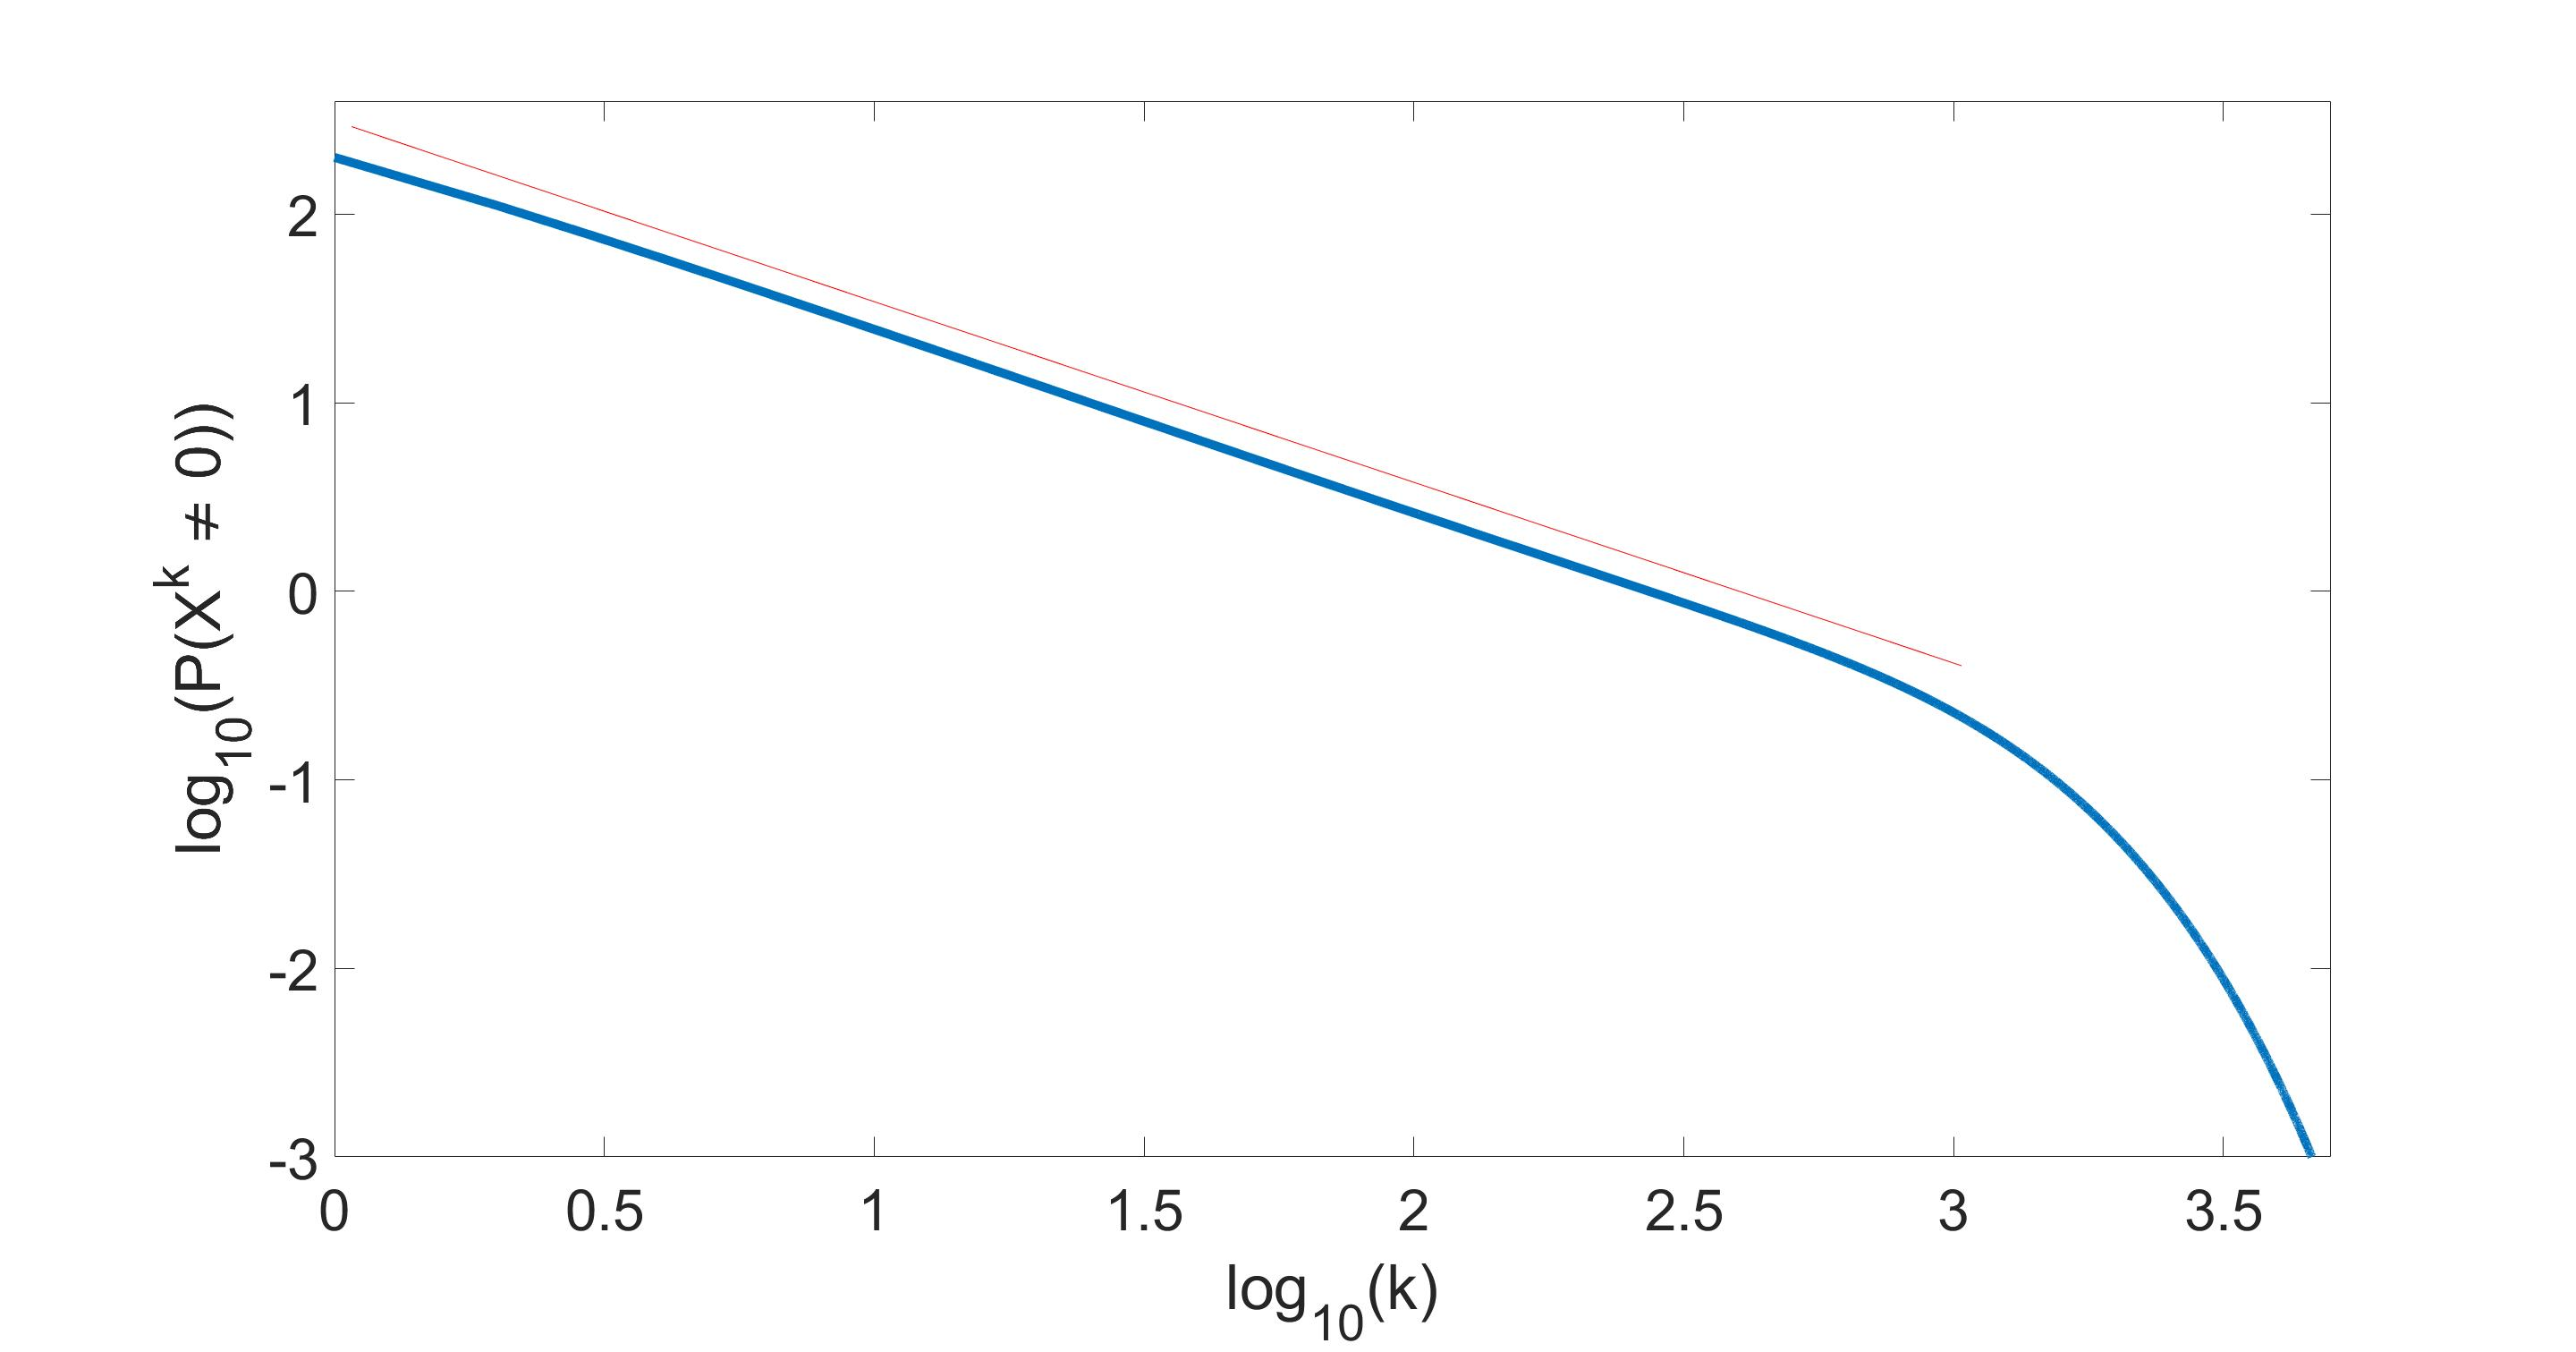
\includegraphics[width=0.5\columnwidth]{power_exp_1.jpg}
	\caption{\textbf{Power law over three orders of magnitude using a clever sum of exponentials.}}
\end{figure}

and we'll even do that thing where we put a straight line next to it, which, I mean, you know, looks kind of like a power law for around 3 orders of magnitude, which is apparently what you "need" to be a valid power law, but that's neither here nor there. What's important here is that the mechanism that determines this very convincing power law shape is actually a power law decay of eigenvalues. So what if we want to change the exponent of this distribution?
\begin{figure}[h!]
	\centering
	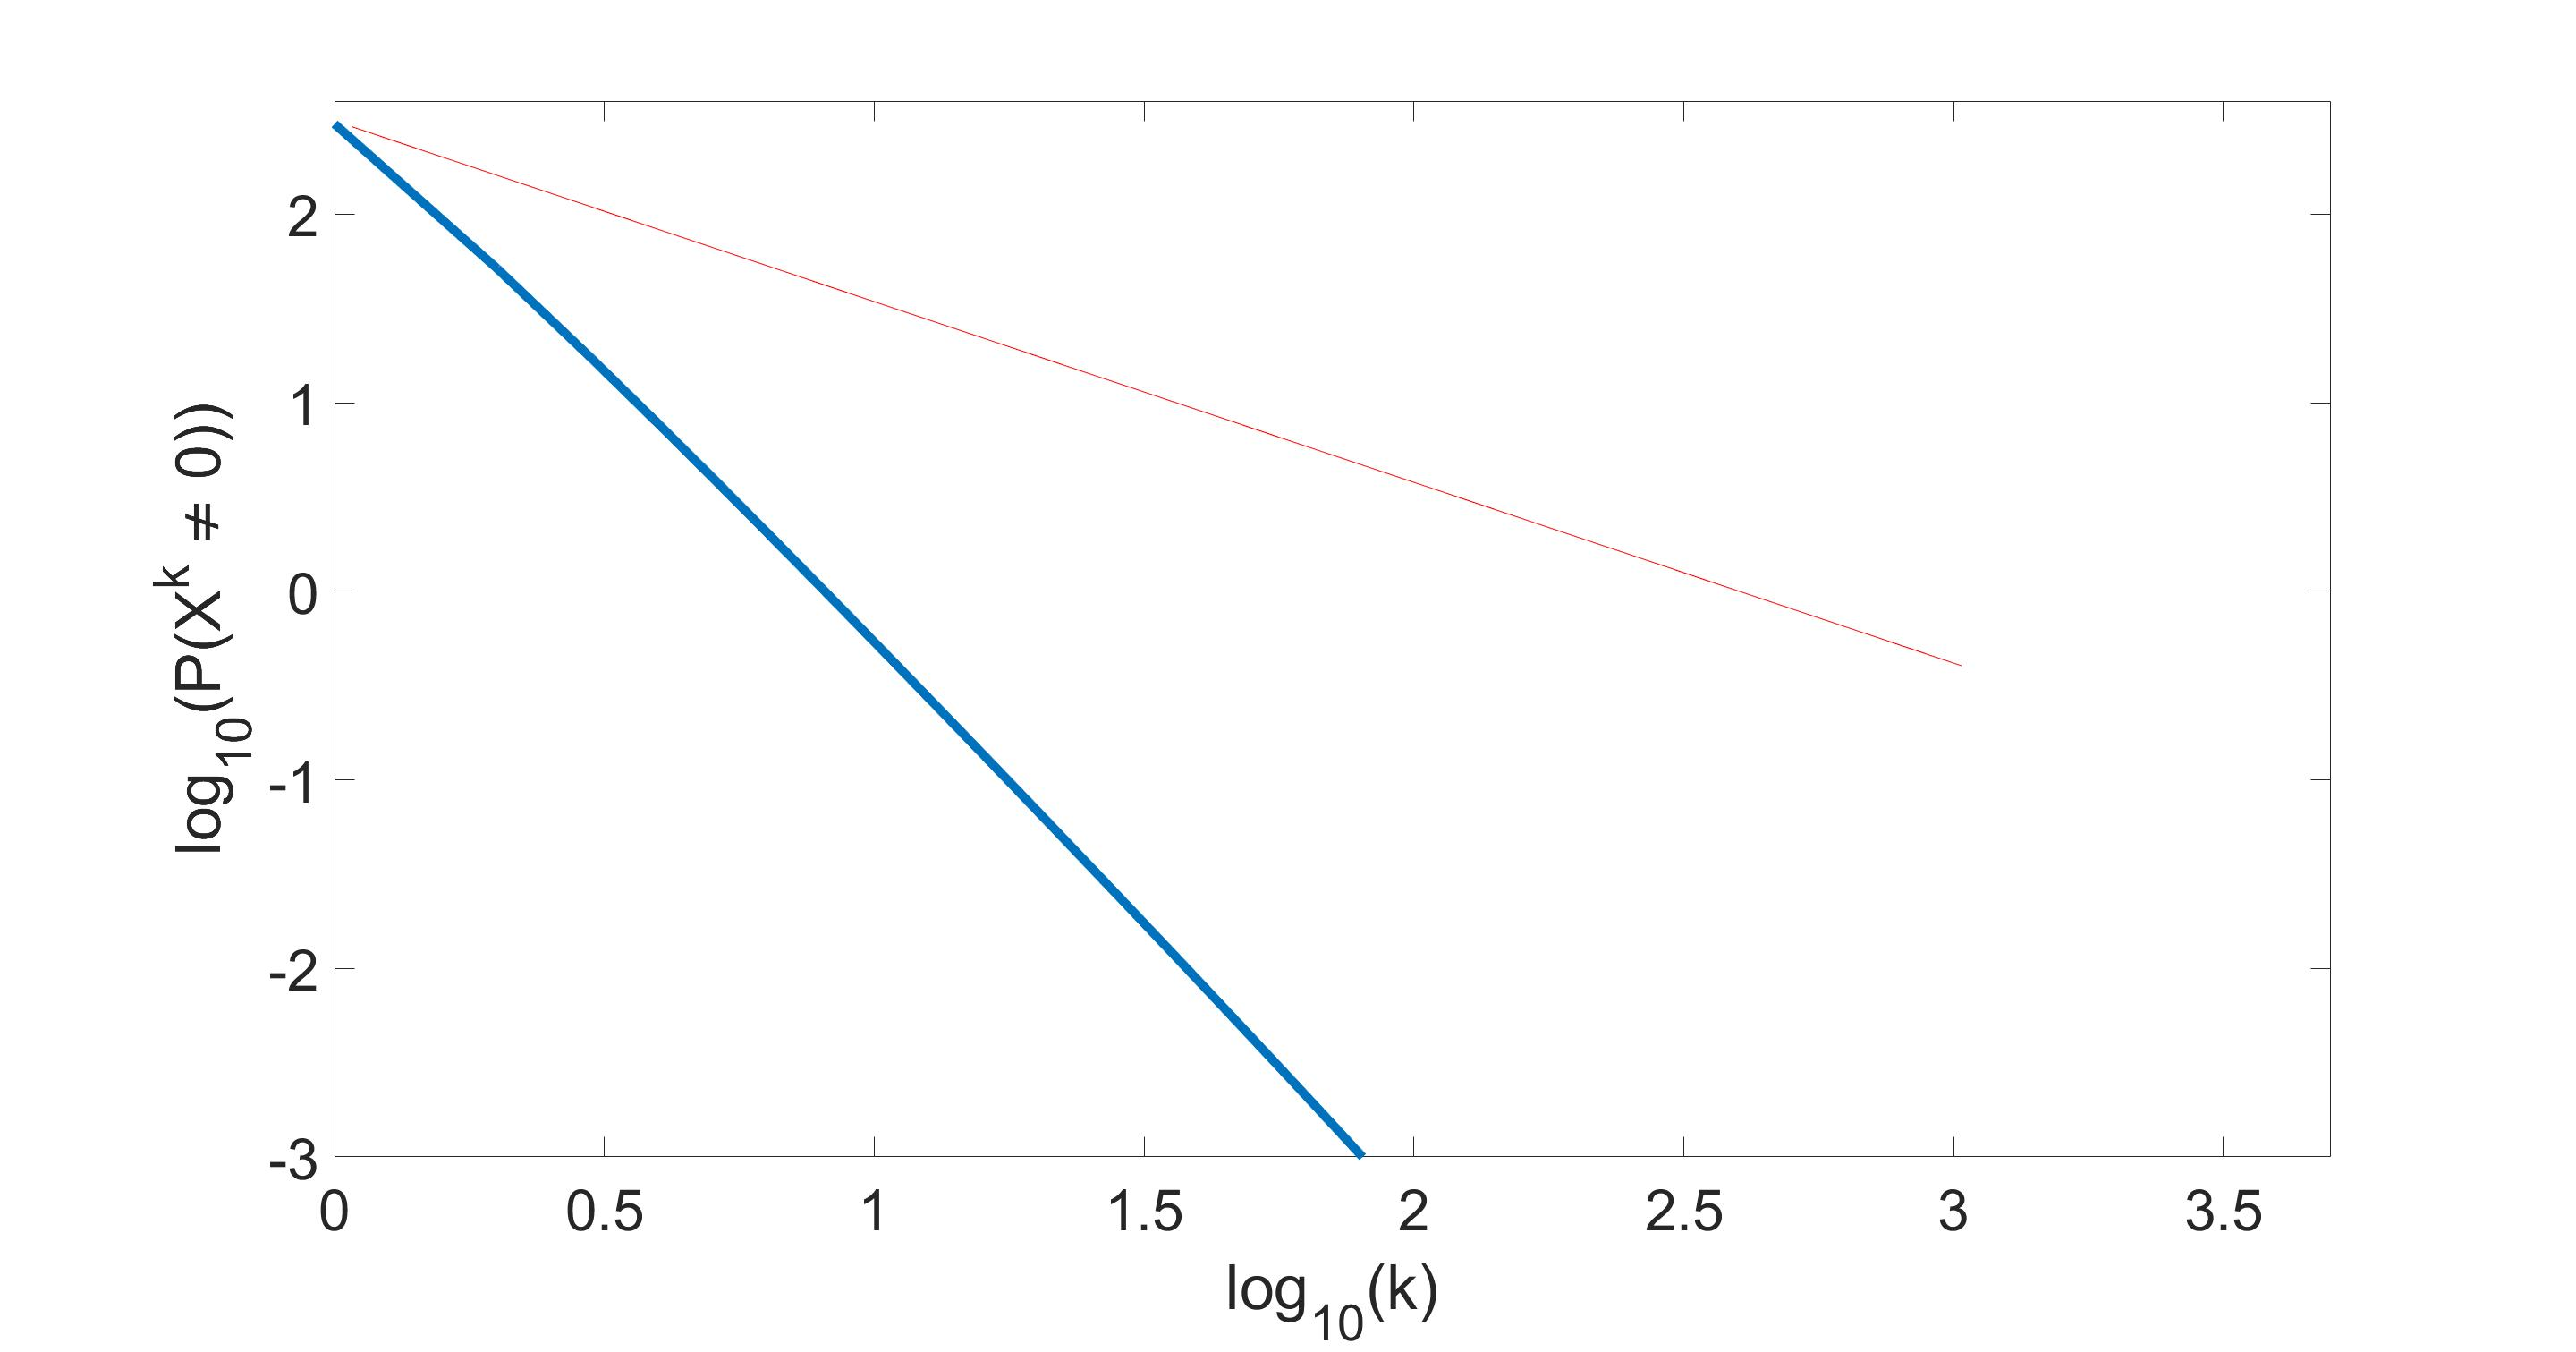
\includegraphics[width=0.5\columnwidth]{power_exp_2.jpg}
	\caption{\textbf{Power law over three orders of magnitude using a clever sum of cleverly weighted exponentials.}}
\end{figure}

Well, we simply have to cleverly pick the coefficients in front of the eigenvalues in order to make the power law more or less steep.
\FloatBarrier





\subsection{Non-Cumulative Avalanche Duration}
Okay okay, so maybe technically the avalanche duration may be given by avalanches that are \emph{exactly} duration $k$, not greater than or equal to $k$. Fine, so we just define a new quantity
\begin{align*}
P(\bm{X}^k \neq \bm{0}) = c_2'(\lambda_2^k - \lambda_2^{k+1}) + c_3'(\lambda_3^k - \lambda_3^{k+1}) + \dotsm + c_N'(\lambda_N^k - \lambda_N^{k+1}),
\end{align*}
which yields the probability of an avalanche that is \emph{exactly} duration $k$. 
\begin{figure}[h!]
	\centering
	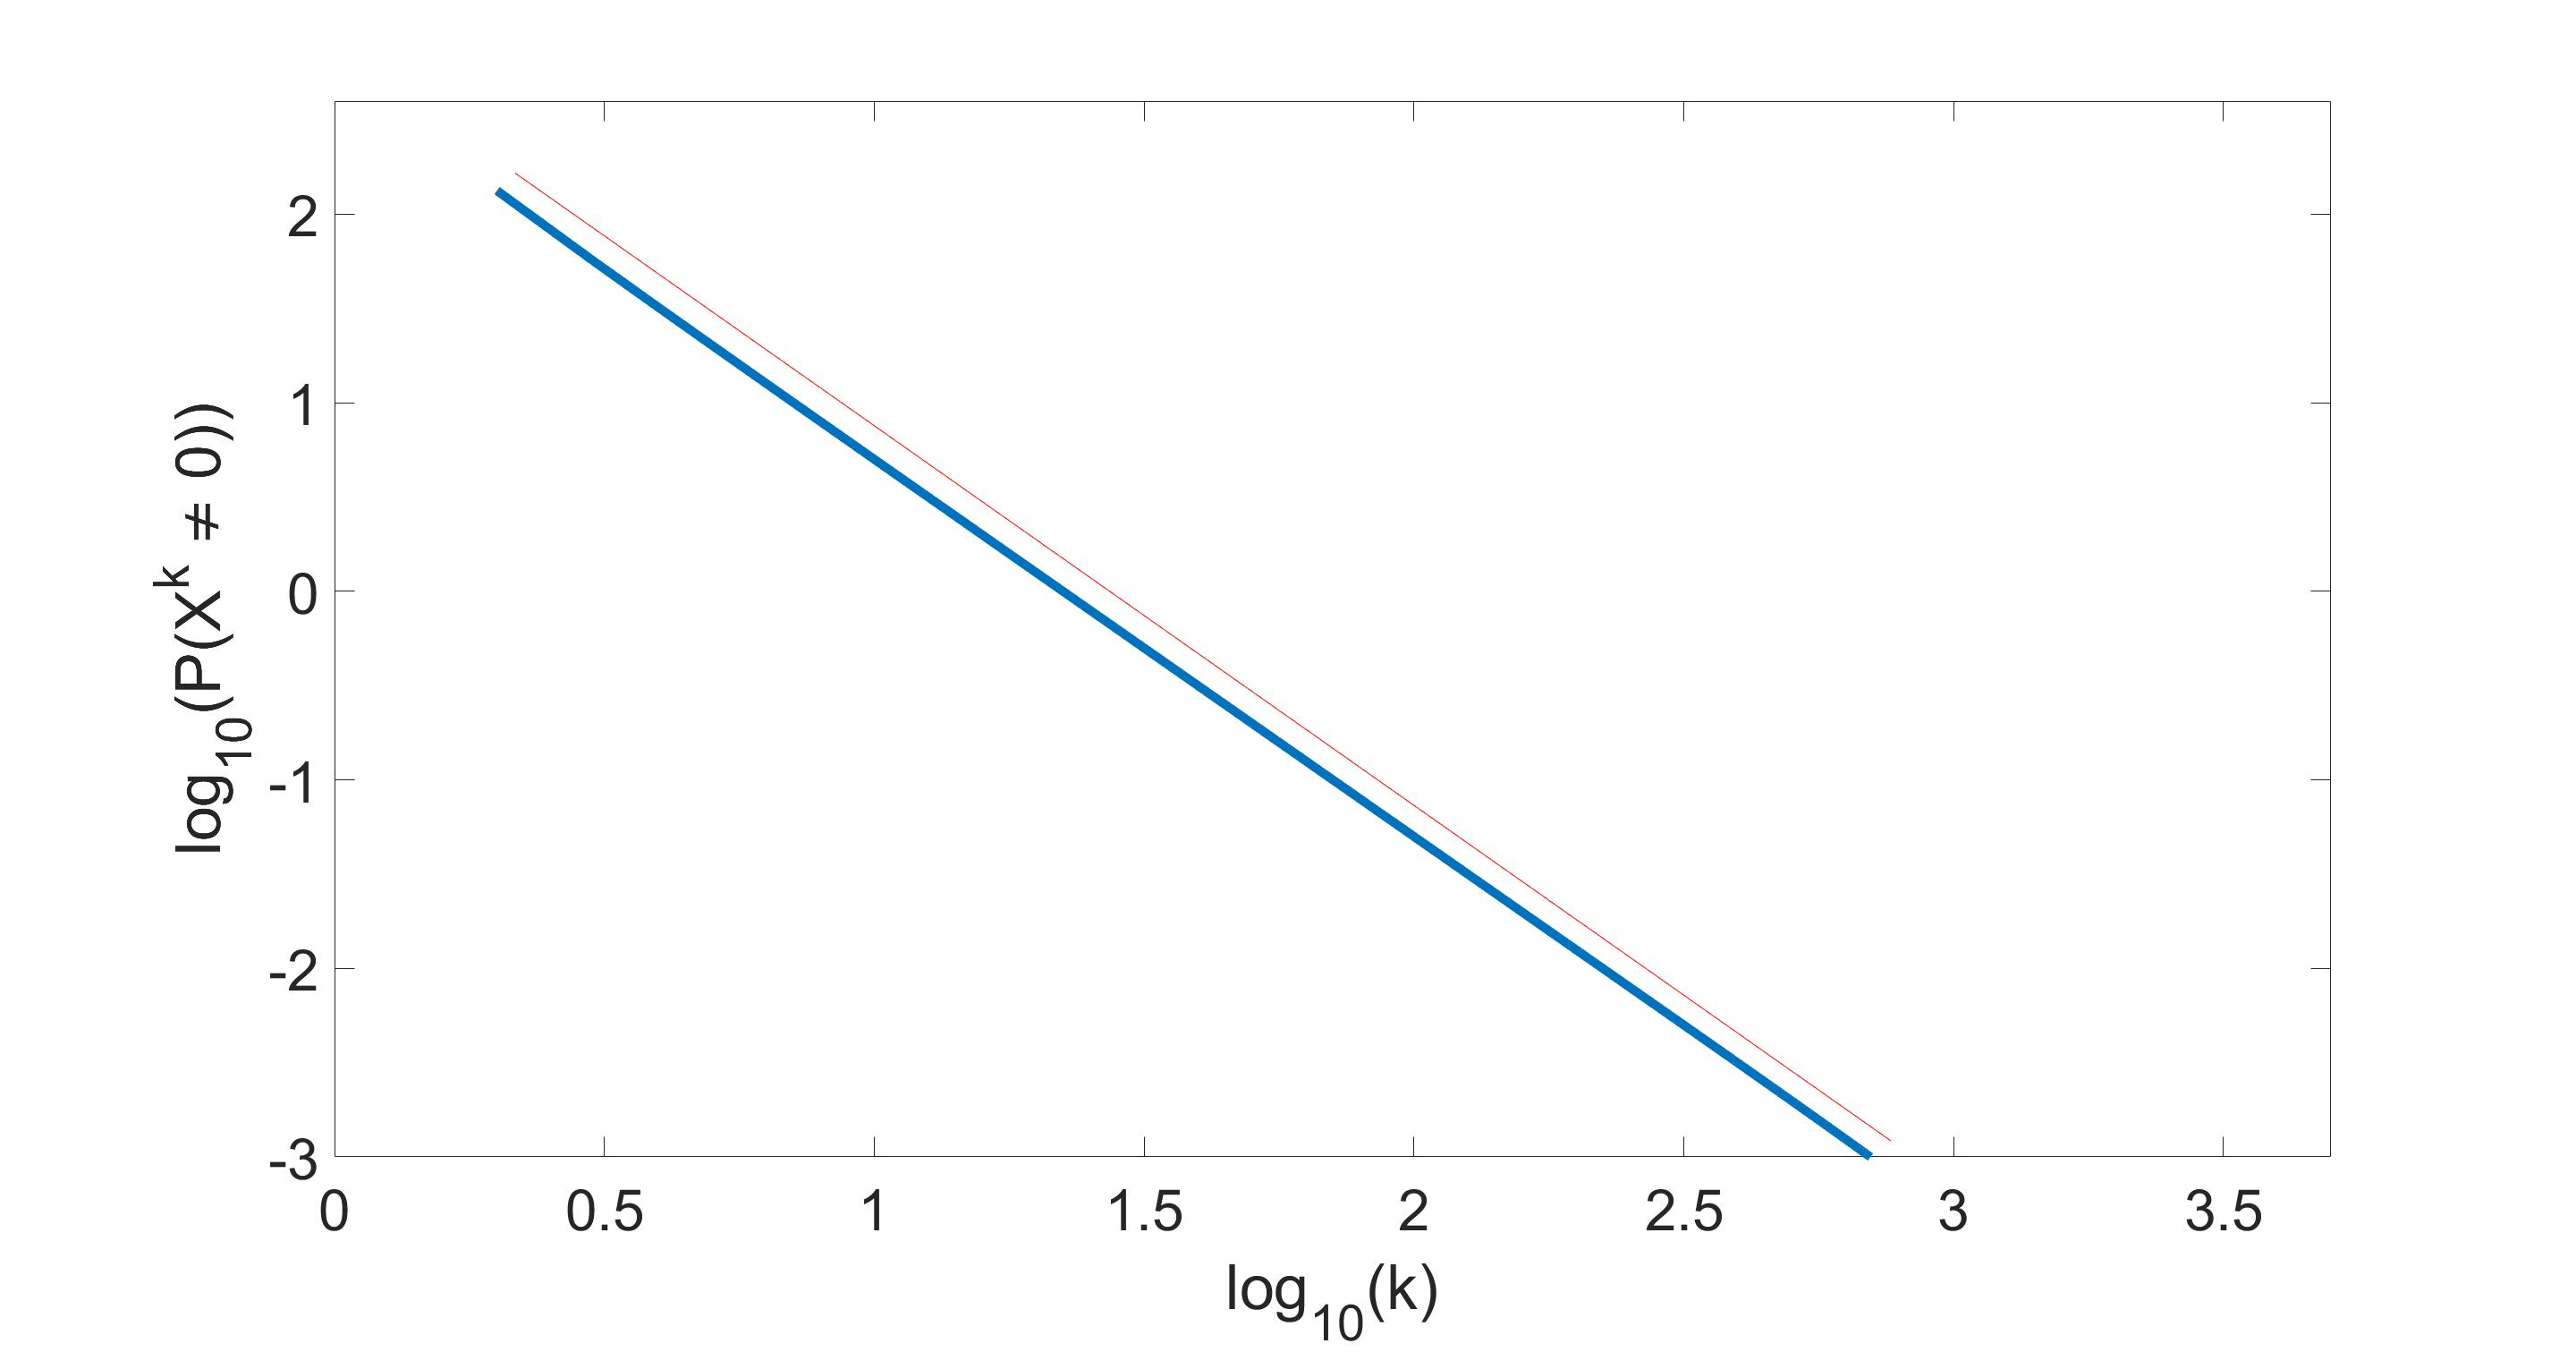
\includegraphics[width=0.5\columnwidth]{power_exp_diff_1.jpg}
	\caption{\textbf{Power law over three orders of magnitude using a clever sum of weighted exponentials.}}
\end{figure}

and of course, picking clever weights,
\begin{figure}[h!]
	\centering
	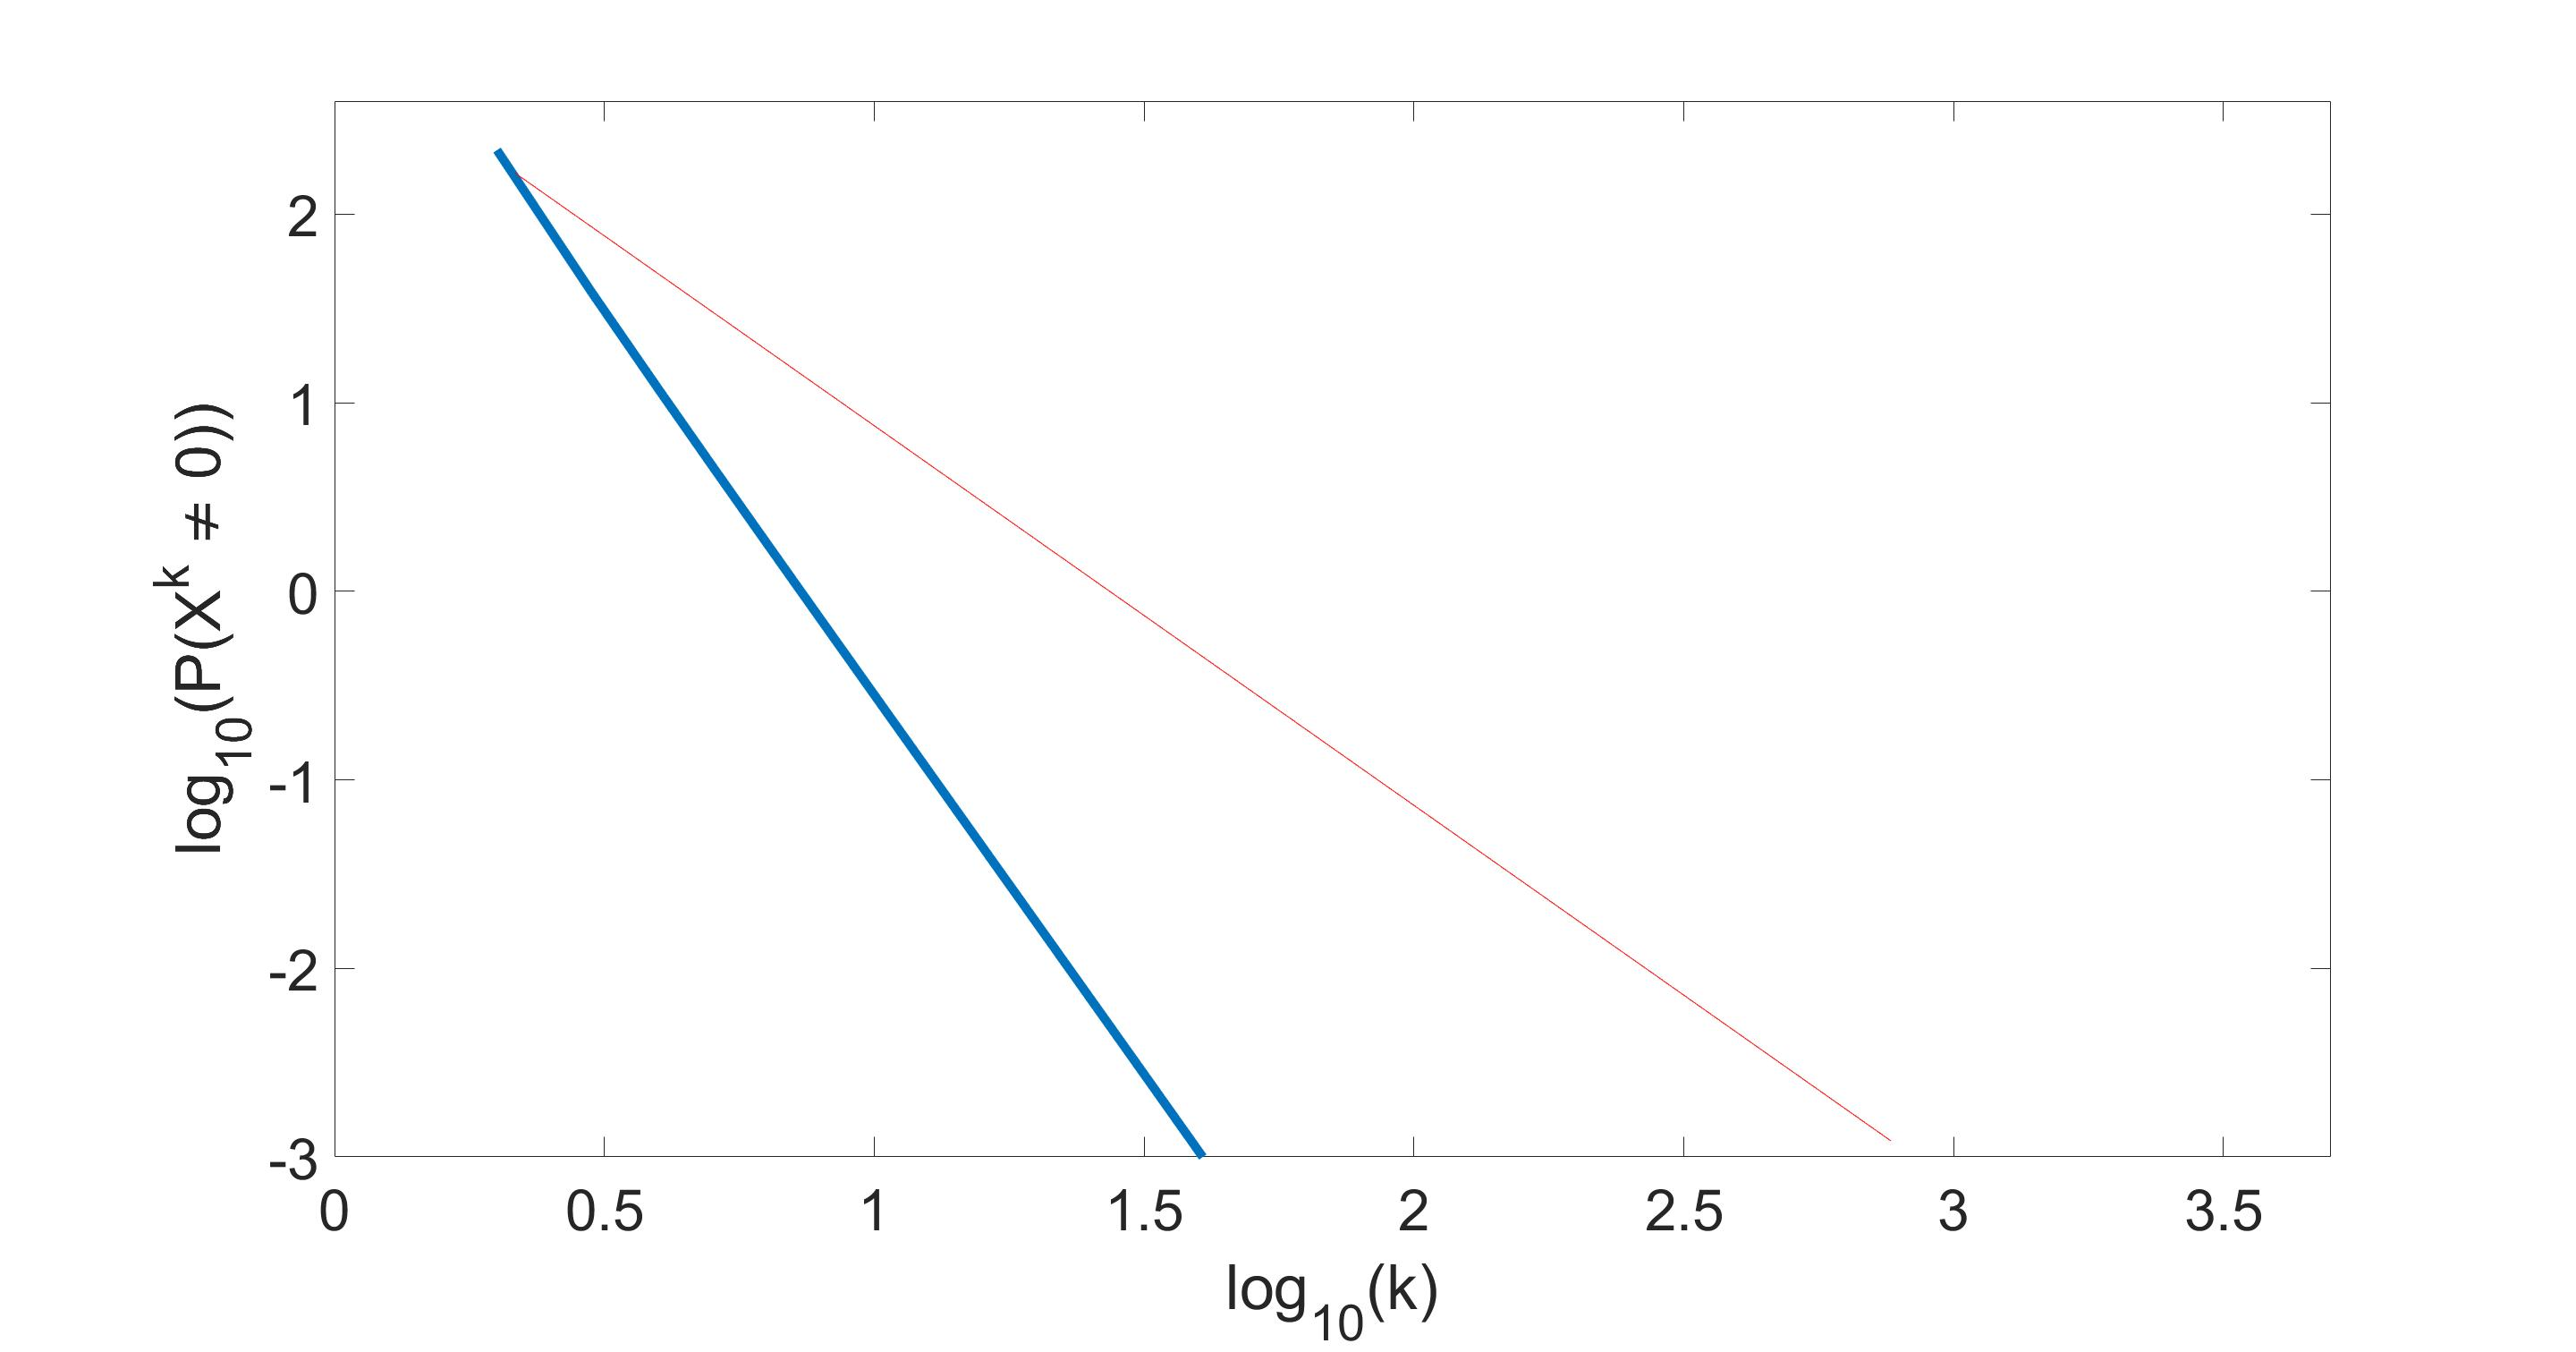
\includegraphics[width=0.5\columnwidth]{power_exp_diff_2.jpg}
	\caption{\textbf{Power law over three orders of magnitude using a clever sum of cleverly weighted exponentials.}}
\end{figure}

Turns out, we can draw our eigenvalues from something other than a power law and still get the same phenomena. What seems to be important is that the eigenvalues decay, that some are close to (but not equal to) 1, and there actually already exists decent literature on approximating power laws with exponential functions. Apparently, "only a handful of exponentials are required in order to approximate a power law up to a given order of magnitude." Ultimately, what we demonstrate here is that power laws in stochastic systems that permit a probability matrix with a zero attractor state most likely arise from a clever selection of eigenvalues and weights.
\FloatBarrier






\subsection{Basic Validation Using Computational Model}
To demonstrate the math is true, we run a simple simulation of stochastic binomial neuronal avalanches for 3 neurons, and plot the probability of survival \emph{versus} avalanche duration. Then, we will take the eigenvalues of the probability matrix and fit this data. As can be seen, and as expected, the probabilities propagated by the eigenvalue powers of the probability matrix match the simulated avalanche duration lengths (over 50000 trials) quite well. 
\begin{figure}[h!]
	\centering
	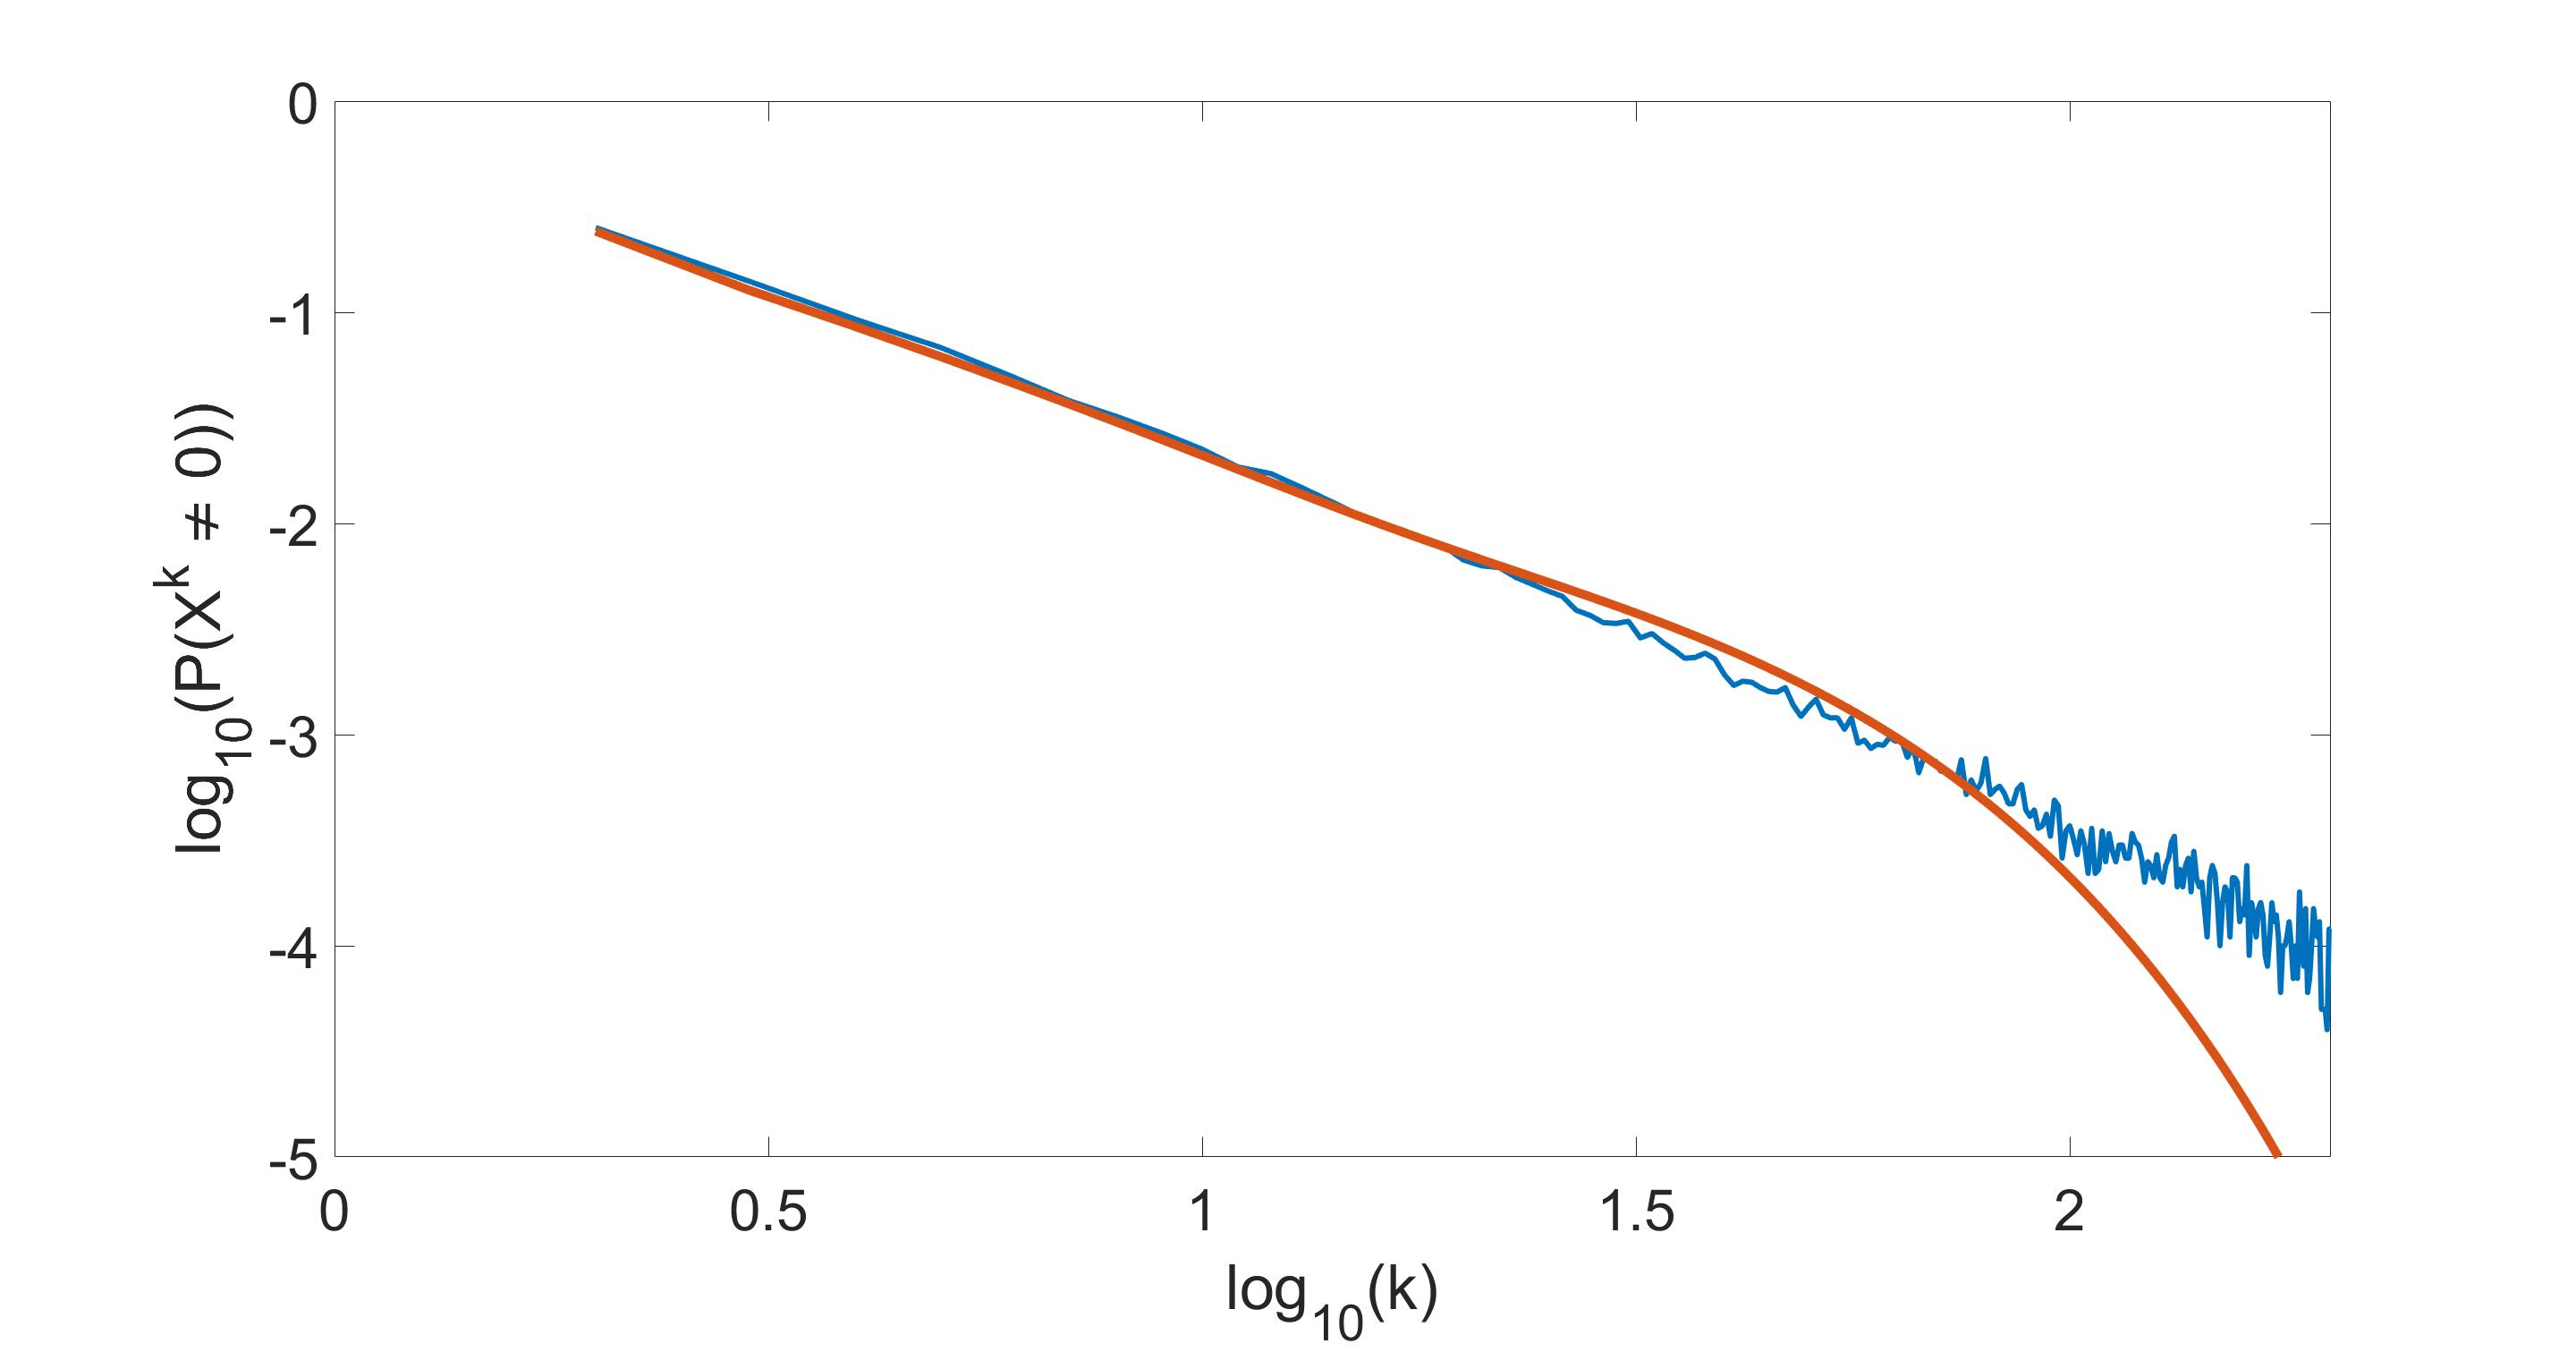
\includegraphics[width=0.5\columnwidth]{power_prob_sim_2.jpg}
	\caption{\textbf{Stochastic binomial spiking model avalanche probability \emph{versus} duration against predicted.}}
\end{figure}
The discrepancy at the tail end arises as a result of... well, probably that we can't construct an infinite by infinite state matrix, or we're estimating the coefficients incorrectly. 






\subsection{Constructing Systems of Arbitrarily Good Power Law Avalanche Duration}
So now that we have some intuition for what features of a probability matrix's eigenvalues yields power laws in avalanche durations, we next seek to contrive systems that yield arbitrarily good power laws. As a demonstration, we create a 9 state Markov process, with probability update rules governed by
\begin{align*}
\prob = 
\begin{bmatrix}
1 & 0.0000 & 0.0000 & 0.0000 & 0.0001 & 0.0000 & 0.0000 & 0.0008 & 0.3541\\
0 & 0.9140 & 0.0000 & 0.0000 & 0.0004 & 0.0000 & 0.0000 & 0.0000 & 0.0000\\
0 & 0.0001 & 0.0000 & 0.0000 & 0.0452 & 0.0001 & 0.0000 & 0.0014 & 0.0000\\
0 & 0.0000 & 0.0000 & 0.9540 & 0.0000 & 0.0000 & 0.0003 & 0.0046 & 0.0000\\
0 & 0.0000 & 0.0000 & 0.0000 & 0.9526 & 0.0000 & 0.0000 & 0.0000 & 0.0000\\
0 & 0.0000 & 0.1209 & 0.0000 & 0.0000 & 0.9992 & 0.0076 & 0.0000 & 0.0001\\
0 & 0.0385 & 0.0045 & 0.0457 & 0.0000 & 0.0000 & 0.2838 & 0.0000 & 0.0000\\
0 & 0.0475 & 0.0413 & 0.0002 & 0.0018 & 0.0007 & 0.0000 & 0.9932 & 0.0003\\
0 & 0.0000 & 0.8333 & 0.0001 & 0.0000 & 0.0000 & 0.7084 & 0.0000 & 0.6455
\end{bmatrix}.
\end{align*}
Yes, I understand that looks a bit large, but bear with me. This matrix was chosen to have eigenvalues best approximating a power law, namely
\begin{align*}
\bm{\lambda} = 
\begin{bmatrix}
0.1353 & 0.6065 & 0.8825 & 0.9692 & 0.9922 & 0.9980 & 0.9995 & 0.9999 & 1
\end{bmatrix}.
\end{align*}
Here's the payoff
\begin{figure}[h!]
	\centering
	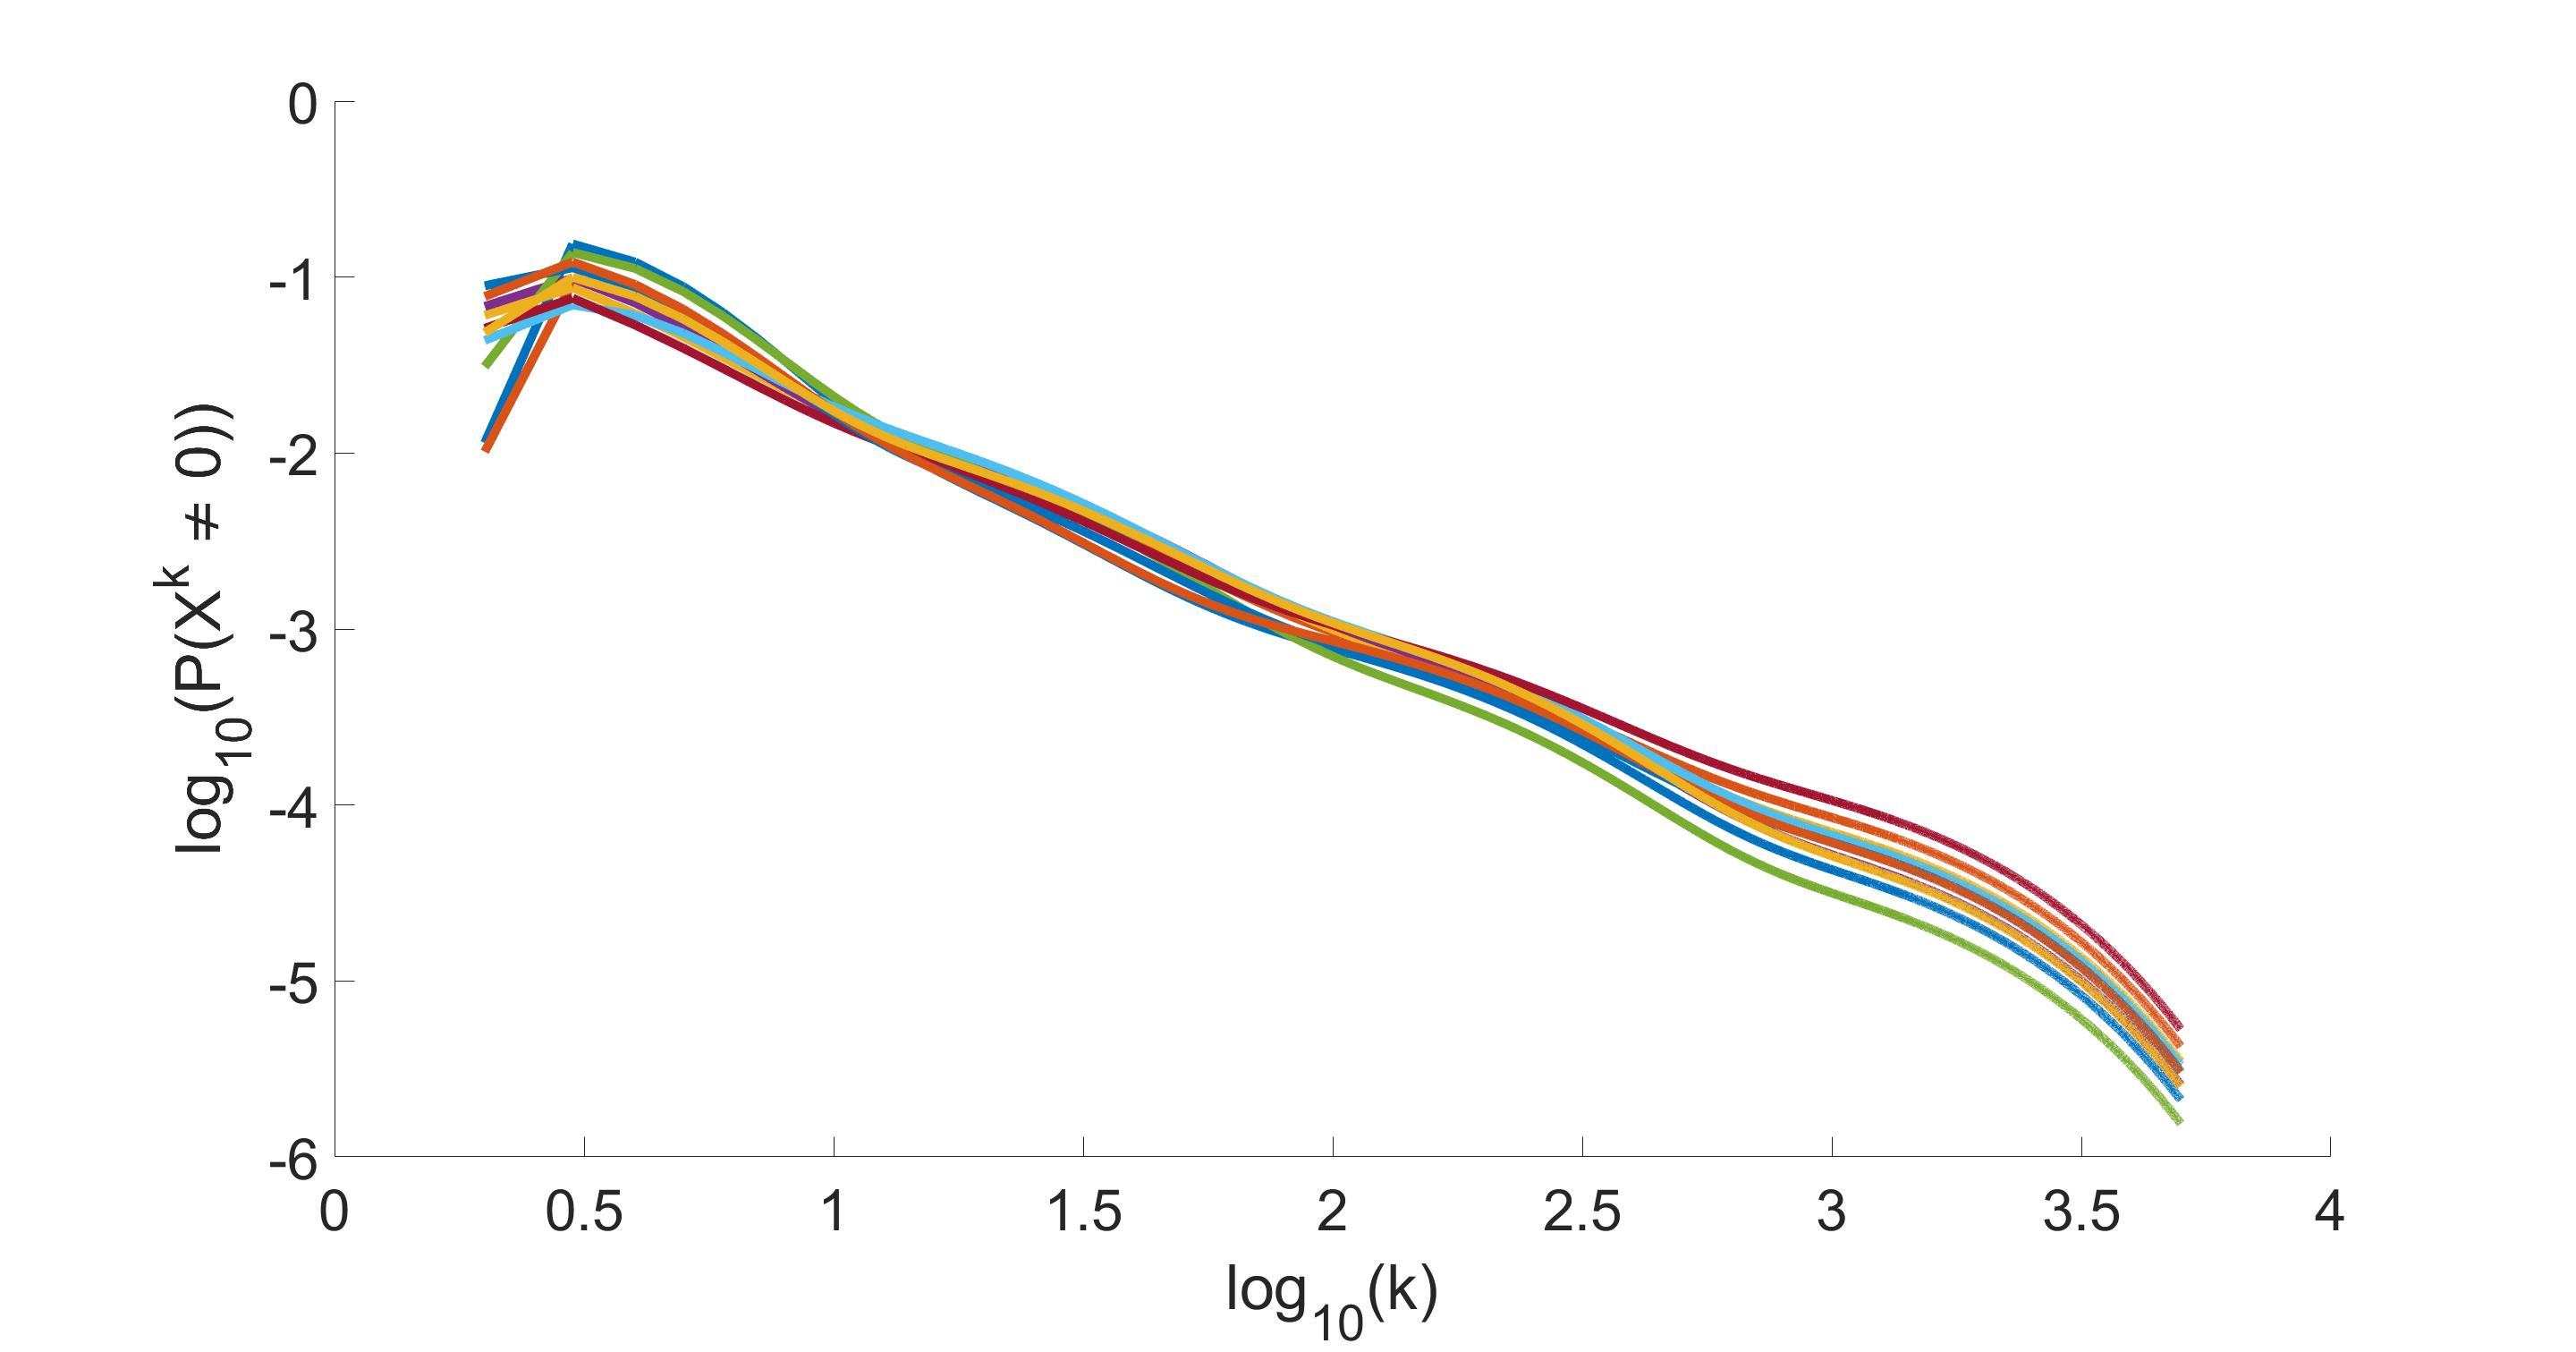
\includegraphics[width=0.5\columnwidth]{power_prob_con_1.jpg}
	\caption{\textbf{Loglog plot of avalanche probability \emph{versus} avalanche duration over 3 decades, 10 initial conditions.}}
\end{figure}

As we can see, our system of 9 states has a pretty beautiful power law distribution of avalanche duration over 3 decades, which is apparently "enough." What's particularly interesting is that our system \emph{literally} has 9 states, one which we consider the zero attractor state indicating the "end" of the avalanche. This power law is also fairly robust to the initial starting probability vector.





\subsection{Summary Statements}
\begin{itemize}
	\item All stochastic processes with one zero attractor state \emph{must} permit a probability matrix $\prob$.
	\item Any such system fundamentally evolves in time as a sum of weighted exponentials.
	\item Power laws in avalanche duration \emph{must} arise as clever sum of cleverly weighted exponentials.
	\item Small, clever systems (e.g. 9 states) demonstrate arbitrarily good power laws over more than 3 decades.
\end{itemize}
\newpage~\newpage







\section{How to Poorly Construct $\prob$}
Now, the reader is thinking, ``this is all fine and good, author, but how can I reliably construct these probability matrices?'' Great question, reader, great question. And you're not really going to like the answer.





\subsection{Really Badly}
Suppose you want your probability matrix to have the following eigenvalues
\begin{align*}
\bm{\lambda} = 
\begin{bmatrix}
1 & 0.9991 & 0.9973 & 0.9918 & 0.9756 & 0.9286 & 0.8007 & 0.5134
\end{bmatrix},
\end{align*}
which are eigenvalues that will yield a nice power law for 3 decades. Well, just make these elements the diagonals of your probability matrix, and let the remaining probabilities decay to zero...
\begin{align*}
\prob_{bad} = 
\begin{bmatrix}
1      & 1-\lambda{2} & 1-\lambda{3} & \dotsm & 1-\lambda{N}\\
0      & \lambda{2}   & 0            & \dotsm & 0\\
0      & 0            & \lambda{3}   & \dotsm & 0\\
\vdots & \vdots       & \vdots       & \ddots & \vdots\\
0      & 0            & 0            & \dotsm & \lambda{N}
\end{bmatrix}.
\end{align*}
Great. So let's push this concept a little further by now considering a system with only 5 states. Not neurons, states.
\begin{figure}[h!]
	\centering
	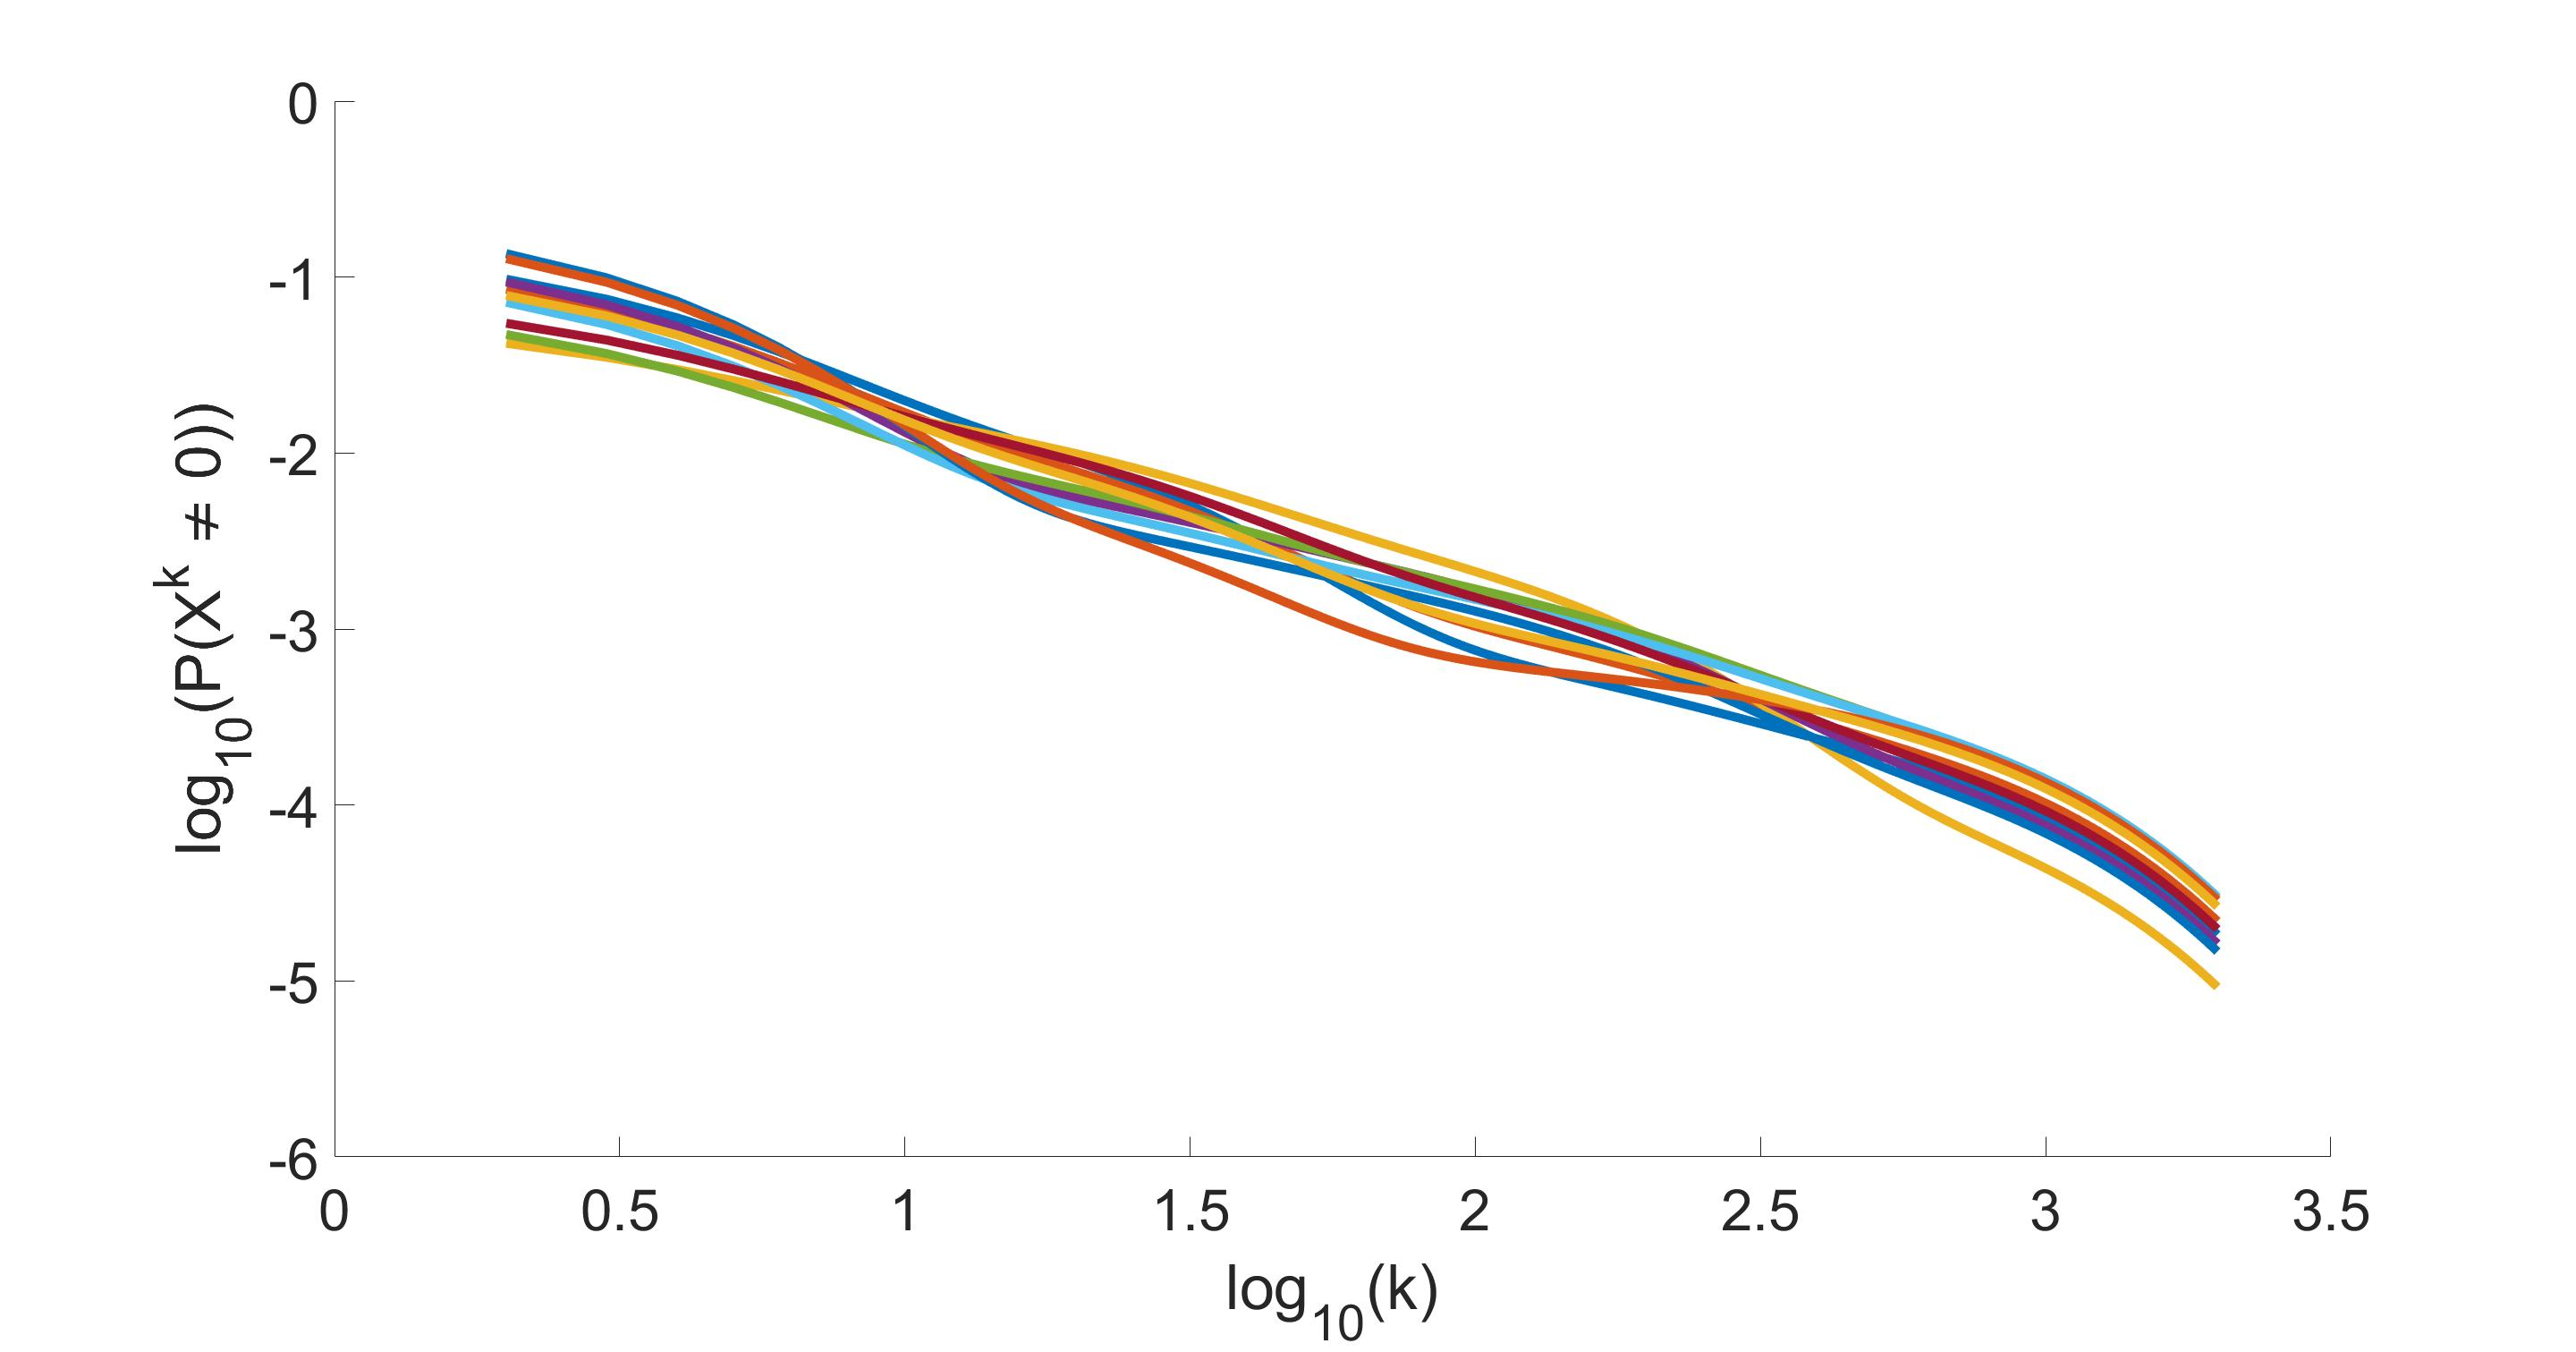
\includegraphics[width=0.5\columnwidth]{power_prob_con_5states.jpg}
	\caption{\textbf{Loglog plot of avalanche probability \emph{versus} avalanche duration for 5 states, 10 initial conditions.}}.
\end{figure}





\subsection{Not As Badly}
It can easily be shown that an upper triangular matrix has eigenvalues equal to the diagonal entries. Hence,
\begin{align*}
\prob_{less-bad} = 
\begin{bmatrix}
1      & p_{21}     & p_{31}     & \dotsm & p_{N1}\\
0      & \lambda{2} & p_{32}     & \dotsm & p_{N2}\\
0      & 0          & \lambda{3} & \dotsm & p_{N3}\\
\vdots & \vdots     & \vdots     & \ddots & \vdots\\
0      & 0          & 0          & \dotsm & \lambda{N}
\end{bmatrix},
\hspace{1in}
\sum_{i=1}^N p_{ji} = 1-\lambda_j.
\end{align*}
This is much better than what we had before. in fact, we've filled in half of the probability matrix, which is more than we can say about the bipartite networks we've dealt with in the past... the figure looks the same as the previous case with just diagonal and zero state entries. So at the end of the day, not the worst possible transition matrices. we can being seeing how we can construct $\prob$ with desired eigenvalues using local probability rules that only define probabilities between states. 





\subsection{Okay, But With More Difficulty}
It can be similarly easily shown that for
\begin{align*}
\prob_{okay} =
\begin{bmatrix}
P_{11} & P_{21} & P_{31} & \dotsm & P_{N1}\\
0      & P_{22} & P_{32} & \dotsm & P_{N2}\\
0      & 0      & P_{33} & \dotsm & P_{N3}\\
\vdots & \vdots & \vdots & \ddots & \vdots\\
0      & 0      & 0      & \dotsm & P_{NN}
\end{bmatrix},
\end{align*}
the eigenvalues of $\prob_{okay}$ are just the set of eigenvalues for $P_{ii}$. So, we capture more entries of our matrix, but the eigenvalues of $\prob_{okay}$ are no longer determined by single probabilities, but instead by matrices. We will now see why this extension is necessary to study any meaningful stochastic system.
\newpage~\newpage





\section{Poorly Linking Local Dynamical Updates To Global Probability}
The reader mumbles ``what a load of mumbo jumbo, who cares about these global probability properties, I'm not God, I can only change a few parameters, not individual entries in the whole probability matrix!'' We hear you, reader, we hear you. Unfortunately, we are also not deities, so here's some contrived mortal intuition instead.






\subsection{Ring Lattice}
Suppose we have a very simple system of $n$ neurons that spike some integer number of times, and are connected cyclically in a directed lattice. Then the update rules are exceedingly simple:
\begin{align*}
X_j^{t+1} &\sim B(X_{j-1}^t, a_{ji})\\
X_1^{t+1} &\sim B(X_n^t, a_{1n}).
\end{align*}
This simplification yields an exceedingly useful property: at any time $t$, if there are $\sum_i x_i^t = s^t$ spikes, then $s^{t+1} \leq s^t$. This is because you can never flip $m$ coins and get \emph{more} than $m$ successes. Why is this property useful? Well, let us again enumerate all possible states of our system (of which there are an infinite number), but this time partition them according to the total number of spikes.
\begin{align*}
S_0 = 
\left\{
\begin{bmatrix}
0 \\ 0 \\ 0 \\ \vdots \\ 0
\end{bmatrix}
\right\},
\hspace{.5in}
S_1 = 
\left\{
\begin{bmatrix}
1 \\ 0 \\ 0 \\ \vdots \\ 0
\end{bmatrix},
\begin{bmatrix}
0 \\ 1 \\ 0 \\ \vdots \\ 0
\end{bmatrix},
\dotsm,
\begin{bmatrix}
0 \\ 0 \\ 0 \\ \vdots \\ 1
\end{bmatrix},
\right\},
\hspace{.5in}
S_2 = 
\left\{
\begin{bmatrix}
1 \\ 1 \\ 0 \\ \vdots \\ 0
\end{bmatrix},
\begin{bmatrix}
2 \\ 0 \\ 0 \\ \vdots \\ 0
\end{bmatrix},
\dotsm,
\begin{bmatrix}
0 \\ 0 \\ 0 \\ \vdots \\ 2
\end{bmatrix},
\right\},
\hspace{.5in}
\dotsm
\end{align*}
and we see that $P(\bm{x}^{k+1} \in S_{m+1} | \bm{x}^k \in S_m) = 0$. Hence, we have our block diagonal matrix $\prob_{okay}$, where each block matrix $P_{ii}$ corresponds to the probability of going from any state in $S_i$ to any other state in $S_i$. All transitions from $S_i \rightarrow S_{i-1}$ don't contribute to the eigenvalues due to the block triangular matrix property outlined previously.

Now, in order for $\bm{x}^t, \bm{x}^{t+1} \in S_i$, we actually require that every spike successfully transmits. We also realize that given a successful outcome, there is only one possible next state in $S_i$, which is simply the rotation matrix $R$ acting on $\bm{x}_i$ such that
\begin{align*}
\bm{x}^{t+1} =
\begin{bmatrix}
0 & 0 & \dotsm & 0 & 1\\
1 & 0 & \dotsm & 0 & 0\\
0 & 1 & \dotsm & 0 & 0\\
\vdots & \vdots & \ddots & \vdots & \vdots\\
0 & 0 & \dotsm & 1 & 0
\end{bmatrix}
\bm{x}^t.
\end{align*}
Hence, we see that we can further divide $S_i$ into sets of period $n$. If $n$ is prime, then we can avoid having smaller groups with harmonic rotation periods. Hence, $P_{ii}$ becomes a block diagonal matrix
\begin{align*}
P_{ii} = 
\begin{bmatrix}
Q_{11} & 0 & \dotsm & 0\\
0 & Q_{22} & \dotsm & 0\\
\vdots & \vdots & \ddots & \vdots\\
0 & 0 & \dotsm & Q_{mm}
\end{bmatrix},
\end{align*}
where each diagonal block $Q_{ii}$ is an $n \times n$ matrix of states that are all rotational transformations of each other. These matrices $Q_{ii}$ now become the diagonal blocks of $\prob$, such that the eigenvalues of $\prob$ are the set of eigenvalues of all $Q_{jj}$ for all $P_{ii}$. Finally, we realize that each $Q_{ii}$ is just the same rotation matrix $R$ with entries weighted by the probability of successfully transmitting all spikes. The eigenvalues of such a rotation matrix all have the same magnitude, given by the $n$th root of the product of its entries. In other words,
\begin{align*}
|\lambda(Q_{ii})| = (q_{12}q_{23}\dotsm q_{n-1 n}q_{n1})^{1/n} = (a_{21}^m a_{32}^m \dotsm a_{n n-1}^m a_{1n}^m)^{1/n}.
\end{align*}
So what are these $q_{ij}$? For $\bm{q}_i, \bm{q}_j \in Q_{kk}$, $Q_{kk} \in P_{mm}$, we have $q_{ij} = P(\bm{x}^{t+1} = \bm{q}_j | \bm{x}^t = \bm{q}_i)$. Because these are rotation sets, every neuron is hit $m$ times for states with a total of $m$ spikes, so $|\lambda(Q_{ii})| = (a_{21}^m a_{32}^m \dotsm a_{n n-1}^m a_{1n}^m)^{1/n} = (a_{21}\dotsm a_{1n})^{m/n}$ with multiplicity $|S_m|$, which, well, can be determined using ideas from mathematics under ``integer partitions''. 

\subsubsection{Simple Case: 2 Neurons}
In a system of two neurons that are connected to each other (with $a = a_{12}a_{21})$ by
\begin{align*}
A = 
\begin{bmatrix}
0      & a_{21}\\
a_{12} & 0
\end{bmatrix},
\end{align*}
we have states
\begin{align*}
S_0 =
\left\{ 
\begin{bmatrix}
0 \\ 0
\end{bmatrix}
\right\},
S_1 =
\left\{ 
\begin{bmatrix}
1 \\ 0
\end{bmatrix},
\begin{bmatrix}
0 \\ 1
\end{bmatrix}
\right\},
S_2 =
\left\{ 
\begin{bmatrix}
2 \\ 0
\end{bmatrix},
\begin{bmatrix}
1 \\ 1
\end{bmatrix},
\begin{bmatrix}
0 \\ 2
\end{bmatrix}
\right\},
S_3 =
\left\{ 
\begin{bmatrix}
3 \\ 0
\end{bmatrix},
\begin{bmatrix}
2 \\ 1
\end{bmatrix},
\begin{bmatrix}
1 \\ 2
\end{bmatrix}
\begin{bmatrix}
0 \\ 3
\end{bmatrix}
\right\},
\dotsm,
\end{align*}
with eigenvalues determined by
\begin{align*}
\bm{\lambda} = 
\begin{bmatrix}
1 & a^{1/n} & a^{1/n} & a^{2/n} & a^{2/n} & a^{2/n} & a^{3/n} & a^{3/n} & a^{3/n} & \dotsm
\end{bmatrix},
\end{align*}
which is, let's be honest, kind of tricky to match to a specific distribution of eigenvalues. This fact also says something very intimate about the nature of avalanche sizes in ring lattices, which is that because $a = \prod_{i=1}^n a_{i i+1}$, the size of the lattice doesn't really change the underlying exponents of system evolution, it simply changes the number of exponents.





\subsubsection{Less Simple Case: $n$ Neurons}
Just to explore this concept a little further, suppose we now have a system of $n$ neurons. What are the possible enumeration of states? Well, $|S_0| = 1$ always.
\begin{align*}
|S_1| &= n\\
|S_2| &= 
\begin{pmatrix}
n\\2
\end{pmatrix}
+ n\\
|S_3| &= 
\begin{pmatrix}
n\\3
\end{pmatrix}
+
2\begin{pmatrix}
n\\2
\end{pmatrix}
+ n,\dotsm,
\end{align*}
etc. As can be seen, the number of eigenvalues representing states of size $1, 2, \dotsm$ become combinatorially huge. All that to say, we can design the eigenvalues of $\prob$ for ring lattices, but we only really have two tuning parameters ($a$ and $n$), which don't easily permit careful eigenvalue distribution tuning. A super interesting caveat of this phenomena is that these eigenvalues are the \emph{true} eigenvalues of the probability matrix $\prob$. Hence, these results hold true for very very large rings. 





\subsection{Feed-Forward Network}
The reader will now exasperatedly admit that yes indeed we have found a matrix for which we can directly relate the matrix entries to the eigenvalues of the probability matrix. Out of sheer hubris and desire to publish (and, of course, the altruistic motive of intellectual curiosity), the reader demands another example.





\subsubsection{Trivial Case: 1 Layer}
Unsurprisingly, a feed-forward network of 1 layer does not really display any interesting dynamics. At any initial state at any time, all activity decays to zero. What does this mean? This means that if the first row of $\prob$ corresponds to the zero state, then $\prob$ is a zero matrix, with all ones in the first row
\begin{align*}
\prob_1 = 
\begin{bmatrix}
1 & \dotsm & 1\\
0 & \dotsm & 0\\
\vdots & \ddots & \vdots\\
0 & \dotsm & 0
\end{bmatrix}.
\end{align*}





\subsubsection{Less Trivial Case: 2 (and eventually $n$) Layers}
With two layers, we can now find an interesting partitioning of states. Intuitively, in any state where the first layer of neurons fired 0 times, any future state cannot have any firing in the first layer. In this way, we define
\begin{align*}
S_2 = 
\begin{bmatrix}
\bm{z}_1\\
\bm{z}_2
\end{bmatrix},
\hspace{1in}
S_1 = 
\begin{bmatrix}
\bm{0}_1\\
\bm{z}_2
\end{bmatrix},
\hspace{1in}
S_0 = 
\begin{bmatrix}
\bm{0}_1\\
\bm{0}_2
\end{bmatrix}
\end{align*}
as our partitions, where $\bm{z}_i$ represents the number of spikes of neurons in layer $i$ excluding the zero state $\bm{0}_i \notin \bm{z}_i$. We note a very interesting property here, where the probabilities $P(\bm{x}^{k+1} \in S_i | \bm{x}^k \in S_{j \leq i}) = 0$. This means that even the diagonal block elements of $\prob$ are also zero.
\begin{align*}
\prob 
&= 
\begin{bmatrix}
P(S_0 \rightarrow S_0) & P(S_1 \rightarrow S_0) & P(S_2 \rightarrow S_0)\\
P(S_0 \rightarrow S_1) & P(S_1 \rightarrow S_1) & P(S_2 \rightarrow S_1)\\
P(S_0 \rightarrow S_2) & P(S_1 \rightarrow S_2) & P(S_2 \rightarrow S_2)\\
\end{bmatrix}\\
&= 
\begin{bmatrix}
1 & P(S_1 \rightarrow S_0) & P(S_2 \rightarrow S_0)\\
0 & 0 & P(S_2 \rightarrow S_1)\\
0 & 0 & 0\\
\end{bmatrix}.
\end{align*}
Here, we have stumbled upon a most unfortunate situation, where this system is actually composed of nontrivial \emph{Jordon Blocks}. Jordon blocks are super bad news bears for us, and can be directly interpreted as divine retribution for our hubris. 
\newpage~\newpage





\section{State-Feedback for Determining Good Initial Probability Distributions}
So this might go a little fast, but bear with me. Recall that we have some rule
\begin{align*}
\bm{X}^{k+1} \sim D(\bm{X}^k, A),
\end{align*}
where the states at the next time step are stochastically drawn from some distribution with some adjacency matrix parameters $A$, and given an enumeration of system states $\bm{x}_i \in X$, where $X$ is the set of all states, and $|X| = N$, we can construct probability matrix $\prob \in \real^{N \times N}$ with some zero attractor state $\bm{x}_0$ such that $p(\bm{x}_0 \rightarrow \bm{x}_0) = 1$. Then given some initial probability distribution of states $\bm{p}_0$, we have
\begin{align*}
\bm{p}^k = \prob^k \bm{p}_0,
\end{align*}
and as always, we care about the eigenvalue distribution of $\prob$. Suppose we consider the new following system
\begin{align*}
\bm{q}^k = \prob^{kT} \bm{q}_0,
\end{align*}
such that the first \emph{row} of $\prob$ has a 1 at the first entry, and zeros for the rest of the entries. Next, consider the following state feedback problem
\begin{align*}
\bm{q}^{k+1} = \prob^T \bm{q}^k + B\bm{b}^k,
\end{align*}
where $\bm{b}^k$ is some control input. If we pick $\bm{b}^k = -K\bm{q}^k$, such that our input is a linear combination of system states, then we get
\begin{align*}
\bm{q}^{k+1} = (\prob^T - BK)\bm{q}^k,
\end{align*}
which is our classic state feedback problem. It turns out that given this state feedback, given our system $(\prob^T, B)$ is controllable, we can arbitrarily place the eigenvalues os $\prob^T-BK$. Hence, if we pick $B$ with all zeros except for the very first entry, then $BK$ only modifies the first row of $\prob^T$. This modification of the first row of $\prob^T$ corresponds directly to picking the transition probabilities \emph{leaving} the zero state, which can be thought of as the picking the initial probability vector $\bm{p}_0$. This basically changes our global probability propagation dynamics to
\begin{align*}
\bm{p}^k = (\prob - (BK)^T)
\begin{bmatrix}
1\\0\\\vdots\\0
\end{bmatrix},
\end{align*}
where we can place the eigenvalues of $\prob - (BK)^T$ where we want using state-feedback.









	
\end{document}
